\chapter{Algorithmes issus de la programmation par contraintes pour le
\CECSP}
\label{sec:PPC_CECSP}
Dans ce chapitre, nous décrivons des algorithmes et modèles issus de
la programmation par contrainte. Les deux premières sections sont
dédiées à la présentation d'algorithmes de filtrage pour le problème
de décision du \CECSP. En effet, comme dans le cas du \CUSP, la
NP-complétude de ce problème implique qu'un algorithme assurant la
cohérence des bornes de chaque variable - assurant l'existence d'une
solution où les valeurs de chaque variables sont comprises dans ces
bornes - ne peut s'exécuter en temps polynomial. Par conséquent,
plusieurs relaxations sont proposées afin de supprimer les valeurs
possibles de début et fin de tâches incohérentes en temps polynomial.

Dans un premier temps, nous montrons que une partie des raisonnements
pour le \CUSP~s'adapte directement au cas du \CECSP. En effet, dans le
\CECSP, une activité peut être vue comme deux sous-activités: 
\begin{itemize}
\item l'une correspondant à une activité rectangulaire, appelée {\it
partie fixe}, dont la date de début et de fin doivent être
déterminées et consommant une quantité $\bmin$ de la ressource;
\item la seconde, appelée {\it partie malléable}, correspondant à une
activité préemptive de même date de début que la partie minimale et
dont chaque partie consomme une quantité de ressource comprise entre
$0$ et $\bmax-\bmin$.
\end{itemize}
La présence d'activités rectangulaires permet alors l'adaptation direct
de certains raisonnement existant pour le \CUSP. Ici, nous
présenterons les adaptations du raisonnement Time-Table, disjonctif et
Time-Table disjonctif. 

Dans un second temps, nous présenterons un nouveau raisonnement
étendu, couplant Time-Table et problème de flots. 

Enfin, une adaptation complète du raisonnement énergétique est décrit
dans le paragraphe~\ref{sec:ER_CECSP}.

Le dernier paragraphe sera quant à lui consacré à la présentation d'un
modèle de programmation par contraintes permettant de résoudre le
\CECSP~ discret, i.e. où les variables ne peuvent prendre que des
valeurs discrètes.

%%% Local Variables:
%%% mode: latex
%%% TeX-master: "../main_file"
%%% End:

\section{Algorithmes de filtrage basés sur le Time-Table}

La section suivante présente plusieurs algorithmes de filtrage pour le
\CECSP. Tous ces algorithmes utilisant une adaptation du Time-Table
pour le \CUSP, nous commençons donc par présenter brièvement comment
ce raisonnement est modifié pour être adapté dans le cadre du \CECSP.
Puis, nous présentons deux autres algorithmes permettant
de réduire l'ensemble des valeurs possibles pouvant être prises par
chaque variable. Le premier est adapté du Time-Table disjonctif pour
le \CUSP~\cite{Gay2015} et le dernier utilise une combinaison entre
problème de flots et profil obligatoire.

\subsection{Le Time-Table}
\index{Time-Table!CECSP}
Comme pour le \CUSP, le Time-Table pour le \CECSP~se base sur la
notion de partie obligatoire des activités, i.e. l'intervalle pendant
lequel une activité est en cours d'exécution dans tous les
ordonnancements réalisables. Cependant, comme dans le cas du \CECSP,
nous ne connaissons pas la durée exacte d'une activité, nous utilisons
une borne inférieure sur sa durée pour calculer la date de début au
plus tard, $\LS$, et la date de fin au plus tôt, $\EE$. Pour calculer
cette borne, remarquons que la configuration permettant de finir une
activité le plus rapidement possible, est celle où l'activité est
exécutée à son rendement maximal $\bmax$. De ce fait, une borne
inférieure sur la durée de l'activité vaut $W_i/f_i(\bmax)$. Nous
pouvons donc calculer la date de début au plus tard de l'activité,
$\LS=d_i-W_i/f_i(\bmax)$, et sa date de fin au plus tôt,
$\EE=r_i+W_i/f_i(\bmax)$. La partie obligatoire d'une activité $i$ est
alors définie de a même manière que pour le \CUSP, i.e la partie
obligatoire de $i$ est l'intervalle $[\LS,\EE]$
(cf. figure~\ref{fig_mand_CECSP}).

Cependant, dans le cas où $\LS \le \EE$, i.e. où l'activité possède
une partie obligatoire, nous pouvons seulement déduire que l'activité
$i$ va consommer au moins une quantité $\bmin$ de la ressource durant
toute sa partie obligatoire, et ce, quelque soit le moment où
l'activité est ordonnancée. La notion de profil obligatoire de la
ressource est donc légèrement différente de celle définie pour le
\CUSP~(cf. définition~\ref{def:profil_oblig},
page~\pageref{def:profil_oblig}).

\begin{defi}
Le profil obligatoire d'une ressource $TT_{\A}$ dans le cas du
\CECSP~est définie de la façon suivante: 
\[TT_{\A}(t)=\sum_{\substack{i \in \A\\\LS \le t \le \EE}} \bmin\quad
  \forall t \in \H\]
Le problème est donc insatisfiable dans le cas où $\exists t \in \H\
:\ TT_{\A}(t) > R$
\end{defi}

\begin{ex}
Considérons l'activité suivante: 

\vspace{-0.5cm}
\begin{center}
  \begin{tabular}{|P{1cm}P{1cm}P{1cm}P{1cm}P{1cm}P{1cm}|}
    \hline
    \ES & \LE & W_i & \bmin & \bmax & f_i(b)\\
    \hline
    1 & 14 & 72 & 2 & 5 & b+3\\
    \hline
  \end{tabular}
\end{center}

Nous pouvons calculer sa date de début au plus tard,
$\LS=d_i-W_i/f_i(\bmax)=14 - 72/8 =5$, ainsi que sa date de fin au
plus tôt, $\EE=r_i+ W_i/f_i(\bmax)=1 + 72/8 =10$. Comme $\EE > \LS$,
l'activité possède une partie obligatoire qui est l'intervalle
$[5,10]$ (voir
figure~\ref{fig_mand_CECSP_a},~\ref{fig_mand_CECSP_b}). Cependant,
nous pouvons seulement en déduire que l'activité sera en cours dans
cet intervalle et ,grâce à la borne inférieure sur la quantité de
ressource que peut consommer l'activité durant son exécution, nous
pouvons déduire que, sur l'intervalle $[\LS,\EE]$, l'activité est au
moins exécutée à $\bmin$ (voir figure~\ref{fig_mand_CECSP_c}).
  
\begin{figure}[htb!]
\vspace{-0.8cm}
\subcaptionbox{Ordonnancement au plus tôt\label{fig_mand_CECSP_a}}[0.3\linewidth]{
    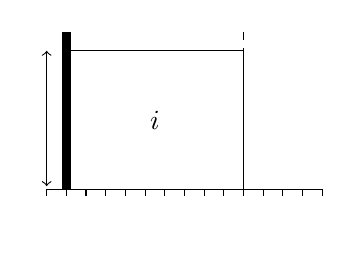
\begin{tikzpicture}
      [xscale=0.25, yscale= 0.4,node distance=0.5cm]
      \node (sil) at (1,0) {} ;
      \node (eil) at (10,0) {} ;
      \node [below of=eil,node distance=0.63cm]  {$\EE$};
      \draw (sil.center) node[below=0.2cm] {$\ES$};
      
      \draw (0,0) -- (14,0);
      \draw[line width=3pt] (1,0) -- (1,5);
      
      \draw[<->] (0,0.1) -- (0,4.4) node[midway,left] {$\bmax$};
      \draw (1,0) rectangle (10,4.4) node[midway] {$i$};

      \draw[dashed] (10,0) -- (10,5);

      \foreach \i in {0,...,14} {
        \draw (\i,0)  -- (\i,-0.2);
      }
    \end{tikzpicture}
}
\hfill
\subcaptionbox{Ordonnancement au plus tard\label{fig_mand_CECSP_b}}[0.3\linewidth]{
    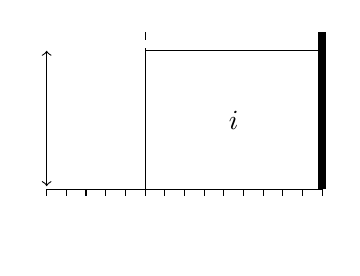
\begin{tikzpicture}
      [xscale=0.25, yscale= 0.4,node distance=0.5cm]
      \node (sir) at (5,0) {} ;
      \node (eir) at (14,0) {} ;
      \node[below of= sir,node distance=0.63cm] {$\LS$};
      \draw (eir.center) node[below=0.2cm] {$\LE$};
      
      \draw (0,0) -- (14,0);
      \draw[line width=3pt] (14,0) -- (14,5);
      
      \draw[<->] (0,0.1) -- (0,4.4) node[midway,left] {$\bmax$};
      \draw (5,0) rectangle (14,4.4) node[midway] {$i$};

      \draw[dashed] (5,0) -- (5,5);

      \foreach \i in {0,...,14} {
        \draw (\i,0)  -- (\i,-0.2);
      }
    \end{tikzpicture}
}
\hfill
\subcaptionbox{Ordonnancement réalisable à $\bmin$ dans
  $[\LS,\EE]$ \label{fig_mand_CECSP_c}}[0.3\linewidth]{ 
    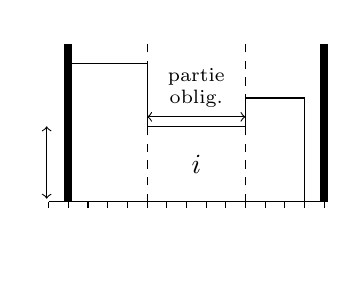
\begin{tikzpicture}
      [xscale=0.25, yscale= 0.4,node distance=0.5cm]
      \node (sir) at (5,0) {} ;
      \node (eil) at (10,0) {} ;
      \node [below of=eil,node distance=0.63cm]  {$\EE$};
      \node[below of= sir,node distance=0.63cm] {$\LS$};
      \draw[<->] (5,2.7) -- (10,2.7) node[midway,above,text width=1.4cm]
      {\begin{center} \scriptsize partie oblig. \end{center}};
      
      \draw[white] (5,0) rectangle (10,2.4) node[midway,color=black] {$i$};
           
      \draw (1,4.4) -- (5,4.4) -- (5,2.4) -- (10,2.4) -- (10,3.3) --
      (13,3.3) -- (13,0);
      
      \draw (0,0) -- (14,0);
      \draw[line width=3pt] (1,0) -- (1,5);
      \draw[line width=3pt] (14,0) -- (14,5);
      
      \draw[<->] (-0.1,0.1) -- (-0.1,2.4) node[midway,left] {$\bmin$};
    


      \draw[dashed] (5,0) -- (5,5);
      \draw[dashed] (10,0) -- (10,5);

      \foreach \i in {0,...,14} {
        \draw (\i,0)  -- (\i,-0.2);
      }
    \end{tikzpicture}
}
\caption{Partie obligatoire d'une activité $i$}
\label{fig_mand_CECSP}
\end{figure}
\end{ex}

Le profil obligatoire peut aussi être calculé en $O(n)$ à l'aide d'un
algorithme de balayage en triant au préalable les activités par date
de début au plus tard et date de fin au plus tôt.

Nous détaillons maintenant l'adaptation du Time-Table disjonctif au
\CECSP. 

\subsection{Le Time-Table disjonctif}

Le second algorithme de filtrage proposé repose sur un raisonnement
appelé Time-Table disjonctif et utilisé, en premier lieu, pour le
\CUSP (cf. paragraphe~\ref{sec:mix_CUSP}). Ce dernier repose sur le
raisonnement Time-Table décrit précédemment et sur le raisonnement
disjonctif.

Le raisonnement disjonctif dans le cadre du \CECSP, est très similaire
à celui défini pour le \CUSP. La différence repose sur la construction
des ensembles disjonctifs. Dans le cas du \CECSP, un couple
d'activités ($i,j)$ sera dit disjonctif si $\bmin+\bmin[j] >R$. Dans
ce cas, nous savons que:
\begin{itemize}
\item l'activité $i$ doit commencer après l'activité $j$, ou, 
\item l'activité $i$ doit finir avant l'activité $j$.  
\end{itemize}

Cette propriété permet, entre autre, d'ajuster la date de début au
plus tôt de $j$. En effet, $\ES[j] \le \EE$ et $\LS \le \EE[j]$
implique que $j$ doit commencer après la fin de l'activité $i$ (voir
figure~\ref{fig:disj_CECSP}). De ce fait, la début de $j$ ne peut arriver
avant la date de fin au plus tôt de $i$, et donc: $\ES[j] \ge \EE$. La
règle de filtrage est ensuite similaire à celle mise en place pour le
\CUSP. 

\begin{reg}
Soient $i, j \in \A, i \neq j$ telles que $\bmin+\bmin[j] < R$ et $\LS
< \EE[j]$. Alors la date de début au plus tôt de l’activité peut être
ajustée et on a : $\ES[j] \ge \EE$.
\end{reg}

\begin{ex}
Considérons les deux activités suivantes: 
\begin{center}
\begin{tabular}{|P{1cm}|P{1cm}P{1cm}P{1cm}P{1cm}P{1cm}P{2cm}|}
    \hline
    act & \ES & \LE & W_i & \bmin & \bmax & f_i(b_i(t))  \\
    \hline
   i & 2 & 11 & 27 & 2 & 3 & 2*b_i(t) +1\\
   j & 1 & 20 & 49 & 2 & 4 & voir fig~\ref{fig:fonct_ CECSP}\\
    \hline
  \end{tabular}
\end{center}

La fonction $f_j(b)$ est définie par l'expression suivante: 
\[f_j(b)=\left\{
\begin{array}{lll}
2b & & b \in [2,3]\\
b+3 & & b \in [3,4]
\end{array}
\right.\] 
et décrite dans la figure~\ref{fig:fonct_CECSP}
\begin{figure}[!htb]
\centering
\begin{tikzpicture}
[xscale=0.8,yscale=0.56]
\node (O) at (1,2) {};
\draw[->] (1,2) -- (5.5,2);
\draw[->] (1,2) -- (1,8);

\path[draw] (2,4) -- (3,6) -- (4,7) ;

\draw[dotted] (2,2) node[below] {\footnotesize $2$} -- (2,8);
\draw[dotted,color=gray!70] (4,2) node[below,color=black] {\footnotesize $4$}
-- (4,8);
\draw[dotted] (3,2) node[below] {\footnotesize $3$} -- (3,8);

\draw (1,4) node[left] {\footnotesize $4$};
\draw (1,6) node[left] {\footnotesize $6$};
\draw (1,7) node[left] {\footnotesize $7$};
\end{tikzpicture}
\caption{Fonction $f_j(b_j(t))$}
\label{fig:fonct_CECSP}
\end{figure}

Dans cet exemple, comme $\bmin +\bmin[j] =4 > 3$, $i$ et $j$ ne
peuvent s'exécuter en parallèle. Si l'activité $i$ finit au temps
$\LE= 11$ alors, elle chevauche forcément l'activité $j $ (voir
figure~\ref{fig:disj_CECSPa} et~\ref{fig:disj_CECSPb}). Dans tous
ordonnancement réalisable, $i$ est donc exécuté avant $j$ et la date de
début au plus tôt de $j$ peut donc être ajustée, i.e. $j$ ne peut
commencer avant $\EE=6$ (voir
figure~\ref{fig:disj_CECSPc}).
  \begin{figure}[htb!] 
    \subcaptionbox{Si $i$ finit au temps $11$...\label{fig:disj_CECSPa}}[0.45\linewidth]{
    \centering
    \begin{tikzpicture} [yscale=0.4,xscale=0.4]   
        \node (O) at (0,0) {};
      \foreach \i in {0,5,...,10} {
        \draw (\i,0) -- (\i,-0.1) node[below] {\small $\i$};
      }
      \fill[gray!50] (2,0) rectangle (11,3.4);
      \fill[gray!50] (1,3.6) rectangle (14,8);
      
      \draw[fill=white] (6.4,0.2) -- (6.4,3.2)   -- (8.4,3.2) -- (8.4,2) --node[midway,below=0.2cm] {$i$}
      (11,2) -- (11,0.2) -- cycle;
      
      \draw[fill=white] (1,3.8) -- (1,7.8)  node[midway,right=0.6cm] {$j$} -- (6,7.8) -- (6,5.8) --
      (9.5,5.8) -- (9.5,3.8) -- cycle;
      \draw[white, pattern=north west lines] (6.4,0) rectangle (9.5,8);

      \draw[->] (0,0) -- (14,0);
      \draw[->] (0,0) -- (0,8) ;
      \draw (0,3) node[left] {$R=3$};
      \draw[densely dotted] (1,-0.1) -- (1,8) node[above] {$\ES[j]$};
      \draw[densely dotted] (8,-0.1) -- (8,8) node[above] {$\EE[j]$};
      \draw[densely dotted] (2,-0.1)  node[below] {$\ES$}-- (2,8);
      \draw[densely dotted] (6,-0.1 ) node[below=0.4cm] {$\EE$}-- (6,8) ;
      \draw[densely dotted] (7,-0.1) node[below] {$\LS$} -- (7,8) ;
      \draw[densely dotted] (11,-0.1) node[below right] {$\LE$} -- (11,8) ;
      \draw[<->] (14.5,0.2) -- (14.5,3.2) node[midway,right] {$\bmax$} ;
      \draw[<->] (14.5,3.8) -- (14.5,7.8) node[midway,right] {$\bmax[j]$} ;   
    \end{tikzpicture}
  }
    \subcaptionbox{...alors $i$ chevauche forcément l'activité $j$\label{fig:disj_CECSPb}}[0.45\linewidth]{
        \centering
        \begin{tikzpicture}[yscale=0.4,xscale=0.4]
      \node (O) at (0,0) {};
      \foreach \i in {0,5,...,10} {
        \draw (\i,0) -- (\i,-0.1) node[below] {\small $\i$};
      }
      \fill[gray!50] (2,0) rectangle (11,3.4);
      \fill[gray!50] (1,3.6) rectangle (14,8);
      
      \draw[fill=white] (7,0.2) rectangle (11,3.2) node[midway]
      {$i$};
      \draw[fill=white] (1,3.8) rectangle (8,7.8) node[midway]
      {$j$};
      \draw[white, pattern=north west lines] (7,0) rectangle (8,8);

      \draw[->] (0,0) -- (14,0);
      \draw[->] (0,0) -- (0,8) ;
      \draw (0,3) node[left] {$R=3$};
      \draw[densely dotted] (1,-0.1) -- (1,8) node[above] {$\ES[j]$};
      \draw[densely dotted] (8,-0.1) -- (8,8) node[above] {$\EE[j]$};
      \draw[densely dotted] (2,-0.1)  node[below] {$\ES$}-- (2,8);
      \draw[densely dotted] (6,-0.1 ) node[below=0.4cm] {$\EE$}-- (6,8) ;
      \draw[densely dotted] (7,-0.1) node[below] {$\LS$} -- (7,8) ;
      \draw[densely dotted] (11,-0.1) node[below right] {$\LE$} -- (11,8) ;
      % \draw[densely dotted] (6,-0.1) -- (6,8) node[above] {$\ES[j]^{'}$};
      % \draw[->] (1.8,5.8) -- (5.2,5.8);
      \draw[<->] (14.5,0.2) -- (14.5,3.2) node[midway,right] {$\bmax$} ;
      \draw[<->] (14.5,3.8) -- (14.5,7.8) node[midway,right]
      {$\bmax[j]$} ;
    \end{tikzpicture}
   }
    \subcaptionbox{$\ES[j]$ peut être ajusté\label{fig:disj_CECSPc}}[\linewidth]{    \centering
      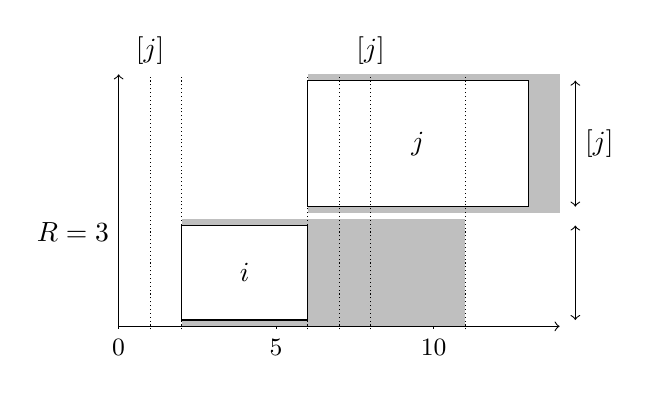
\begin{tikzpicture} [yscale=0.4,xscale=0.4]
      \node (O) at (0,0) {};
      \foreach \i in {0,5,...,10} {
        \draw (\i,0) -- (\i,-0.1) node[below] {\small $\i$};
      }
      \fill[gray!50] (2,0) rectangle (11,3.4);
      \fill[gray!50] (6,3.6) rectangle (14,8);
      
      \draw[fill=white] (2,0.2) rectangle (6,3.2) node[midway]
      {$i$};
      \draw[fill=white] (6,3.8) rectangle (13,7.8) node[midway]
      {$j$};

      \draw[->] (0,0) -- (14,0);
      \draw[->] (0,0) -- (0,8) ;
      \draw (0,3) node[left] {$R=3$};
      \draw[densely dotted] (1,-0.1) -- (1,8) node[above] {$\ES[j]$};
      \draw[densely dotted] (8,-0.1) -- (8,8) node[above] {$\EE[j]$};
      \draw[densely dotted] (2,-0.1)  node[below] {$\ES$}-- (2,8);
      \draw[densely dotted] (6,-0.1 ) node[below=0.4cm] {$\EE$}-- (6,8) ;
      \draw[densely dotted] (7,-0.1) node[below] {$\LS$} -- (7,8) ;
      \draw[densely dotted] (11,-0.1) node[below right] {$\LE$} -- (11,8) ;
      \draw[<->] (14.5,0.2) -- (14.5,3.2) node[midway,right] {$\bmax$} ;
      \draw[<->] (14.5,3.8) -- (14.5,7.8) node[midway,right] {$\bmax[j]$} ;

  \end{tikzpicture}
}
  \caption{Raisonnement disjonctif}
  \label{fig:disj_CECSP}
\end{figure}
\end{ex}

Nous pouvons maintenant présenter l'adaptation du Time-Table
disjonctif au cas du \CECSP. Pour ce faire, nous commençons par
adapter la définition d'intervalle minimum de superposition, puis nous
présenterons les modifications apportées aux règles d'ajustement du
\CUSP~afin que ces dernières soient applicables dans le cas du
\CECSP. Enfin, l'extension de ces règles dans le cas où les activités
ne possèdent pas de partie obligatoire sera décrit. Cette extension
n'avait pas été présentée dans le chapitre sur le \CUSP~mais est
décrite dans l'article~\cite{Gay2015}. 

La notion d'intervalle minimum de superposition s'adapte naturellement
au cas du \CECSP. En effet, cette intervalle représente l'ensemble
minimal de points de temps tel que une activité $i$ est forcément en
cours durant un de ces points. 

\begin{defi}
\label{des:moi_CUSP} 
Soit $\EE^{-}$ le point le plus proche de $\EE$, i.e. $\forall \delta
>0 , |\EE^{-} -\EE| \le \delta$. L'intervalle minimum de
superposition d'une activité $i$,noté $moi_i$, est alors défini par
$moi_i=[\EE^{-},\LS{]}$ si $i$ ne possède pas de partie obligatoire et
$moi_i=\emptyset$ sinon.   

Il s'agit du plus petit intervalle de temps tel que $i$ s’exécute au
moins durant un point de temps de cet intervalle, et ce peu importe le
moment auquel l'activité $i$ est exécutée.
\end{defi}


\begin{ex}
La figure~\ref{fig:moi_CECSP} illustre l'intervalle minimum de
superposition d'une activité $i$ ne possédant pas de partie
obligatoire. En effet, quelque soit la position de l'activité $i$,
elle intersecte forcément $moi_i$.
\begin{figure}[!htb]
  \begin{center}
    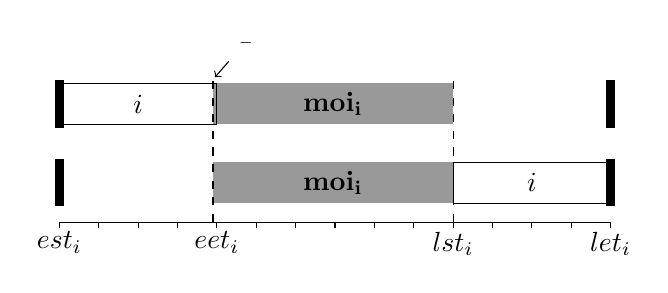
\begin{tikzpicture}
      [xscale=0.5, yscale= 0.4,node distance=0.5cm][decoration={brace}]
      \node (sil) at (0,0) {} ;
      \node (sir) at (10,0) {}; 
      \draw (10,0) node[below] {$lst_i$};
      \node (eir) at (14,0) {} ;
      \node (eil) at (4,0) {} ;
      \draw (4,0) node [below]  {$eet_i$} ;
      \draw (sil.center) node[below] {$est_i$}--
      (eir.center) node[below] {$let_i$};
      
      \draw[<-] (3.95, 4.6) -- (4.3,5.1) node[above=0.2cm,right] {\scriptsize $\EE^{-}$};
      \draw[line width=3pt] (0,0.5) -- (0,2);
      \draw[line width=3pt] (14,0.5) -- (14,2);
      \draw[line width=3pt] (0,3) -- (0,4.5);
      \draw[line width=3pt] (14,3) -- (14,4.5);

      \fill[gray!80] (3.9,0.6) rectangle (10,1.9) node[midway,color=black] {$\mathbf{moi_i}$};
      \fill[gray!80] (3.9,3.1) rectangle (10,4.4) node[midway,color=black] {$\mathbf{moi_i}$};
      
      \draw (0,3.1) rectangle (4,4.4) node[midway] {$i$};
      \draw (10,0.6) rectangle (14,1.9) node[midway] {$i$};

      \draw[dashed] (3.9,0) -- (3.9,4.5);
      \draw[dashed] (10,0) -- (10,4.5);

      \foreach \i in {0,...,14} {
        \draw (\i,0)  -- (\i,-0.2);
      }
    \end{tikzpicture}
  \end{center}

  \caption{Intervalle minimum de superposition d'une activité}
  \label{fig:moi_CECSP}
\end{figure}
\end{ex}

Afin de pouvoir adapter le raisonnement au cas du \CECSP, 
\subsection{Le Time-Table basé sur les flots}




\section{Algorithme de filtrage du raisonnement énergétique}
\label{sec:ER_CECSP}

La section ci-dessous décrit l'adaptation du raisonnement
énergétique, introduit dans~\cite{RELopez} pour la contrainte cumulative,
et décrit dans la sous-section~\ref{sec:cumu_propag}. Nous commençons,
dans un premier temps, par décrire l'algorithme de vérification de ce
raisonnement, puis nous présenterons les règles d'ajustements qui
peuvent être mises en place pour filtrer les domaines des
variables. Enfin, la dernière partie de cette section sera consacrée à
la caractérisation des intervalles d'intérêt pour l'algorithme de
vérification et pour les règles d'ajustement.

\subsection{Algorithme de vérification}

\subsubsection{Condition nécessaire d'existence de solution}
Pour décrire l'algorithme de vérification, nous rappelons d'abord
l'idée principale sur laquelle repose le raisonnement énergétique. Le
principe est donc, étant donné un intervalle $[t_1,t_2[$, de calculer
les consommations minimales de ressource des activités dans cet 
intervalle et de les comparer à la quantité de ressource disponible
dans ce même intervalle. Si la ressource disponible n'est pas
suffisante pour ordonnancer les consommations minimales de toutes les
activités, une incohérence est détectée.

Dans le cas du \CUSP, la quantité de ressource requise par une
activité pouvait être calculée de manière directe. Ici, ce calcul sera
fait en deux fois: nous calculons d'abord la quantité d'énergie
requise par une activité à l'intérieur de l'intervalle $[t_1,t_2{[}$,
notée $\wb$, puis nous traduisons cette énergie en une quantité de
ressource, notée $\bb$. Ceci nous permettra ensuite de la comparer
avec la ressource disponible dans $[t_1,t_2{[}$.

Formellement, ces quantités sont représentées par les expressions
suivantes: 
\begin{align}
  \wb= \min \int_{t_1}^{t_2} f_i(b_i(t))dt & & \text{sous 
                                               \eqref{tw_CECSP}-\eqref{nrj_CECSP}}\\
  \bb= \min \int_{t_1}^{t_2} b_i(t)dt & & \text{sous 
                                          \eqref{tw_CECSP}-\eqref{nrj_CECSP}} \label{eq:minConso}
\end{align}

Comme pour le cas du \CUSP, la fonction de marge, notée $SL(t_1,t_2)$,
permet de mesurer l'écart entre la quantité de ressource disponible et
les consommations minimales de toutes les tâches dans l'intervalle
${[}t_1,t_2{]}$. Cette fonction est définie de la manière suivante:
\[ SL(t_1,t_2)=R(t_2-t_1)-\sum\limits_{i \in A} \bb \]

Ceci nous permet d'énoncer la condition nécessaire d'existence
d'une solution qui est à la base de l'algorithme de vérification du
raisonnement énergétique:

\begin{theo}
  \label{th:ER_CECSP}
  Soit $\I$ une instance du \CECSP. S'il existe $t_1 < t_2 \in
  \mathbb{R}^2$ tel que $SL(t_1,t_2) <0$ alors $\I$ ne peut pas avoir
  de solution.
\end{theo}

\begin{proof}
  Par l'absurde, supposons qu'il existe $t_1 < t_2 \in \mathbb{R}^2$ tel
  que $SL(t_1,t_2) <0$ et que l'instance $\I$ soit satisfiable. Par
  définition, $\bb$ est la quantité de ressource minimale que doit
  consommer l'activité $i$ dans l'intervalle $[t_1,t_2{[}$. 

  Donc, dans toute solution réalisable, nous avons: 
  \begin{align*}
    & \int_{t_1}^{t_2} b_i(t)dt \ge \bb\\
    \Rightarrow  & \sum_{i \in \A} \int_{t_1}^{t_2} b_i(t)dt \ge \sum_{i
                   \in \A}  \bb > R(t_2-t_1)
  \end{align*}
  Et ceci contredit le fait que $\sum_{i \in \A} b_i(t) \le
  R(t_2-t_1)$. 
\end{proof}

Dans un premier temps, nous allons nous intéresser au calcul de $\wb$,
le calcul de $\bb$ sera détaillé dans un second temps. 


\subsubsection{{\'E}nergie minimale dans un intervalle}

Pour calculer $\wb$, nous analysons les différentes configurations de
la consommation minimale d'une activité. Remarquons que les
configurations conduisant à une consommation minimale dans
l'intervalle $[t_1,t_2{[}$ sont celles où l'activité est ordonnancée à
$\bmax$ à l'extérieur de cet intervalle. Ces configurations, décrites
dans la figure~\ref{fig:conso_CECSP}, peuvent être regroupées en trois
catégories:
\begin{itemize}
\item l'activité est {\it calée à
    gauche} (figure~\ref{fig:conso_CECSPa}, \ref{fig:conso_CECSPb},
  \ref{fig:conso_CECSPd} et \ref{fig:conso_CECSPg}): l'activité démarre
  à $\ES$ et est ordonnancée à $\bmax$ pendant l'intervalle
  $[\ES,t_1{[}$;
\item l'activité est {\it calée à
    droite} (figure~\ref{fig:conso_CECSPb}, \ref{fig:conso_CECSPc},
  \ref{fig:conso_CECSPf} et \ref{fig:conso_CECSPi}): l'activité finit à
  $\LE$ et est ordonnancée à $\bmax$ pendant l'intervalle $[t_2,\LE{[}$;
\item l'activité est {\it centrée} (figure~\ref{fig:conso_CECSPe} et
  \ref{fig:conso_CECSPh}): l'activité occupe tout l'intervalle
  $[t_1,t_2[$, soit en étant ordonnancée à $\bmax$ pendant l'intervalle
  $[\ES,t_1{[} \cup [t_2,\LE{[}$, soit en étant ordonnancée à $\bmin$
  durant tout l'intervalle $[t_1,t_2{[}$.

  En effet, lorsque l'activité est ordonnancée à $\bmax$ pendant
  l'intervalle $[\ES,t_1{[} \cup [t_2,\LE{[}$, il peut arriver que la
  quantité d'énergie restant à apporter à l'activité durant l'intervalle
  $[t_1,t_2[$ ne soit pas suffisante pour assurer la satisfaction de la
  contrainte de consommation minimale~\eqref{req_CECSP}. Le cas où
  l'activité est ordonnancée à $\bmin$ durant tout l'intervalle
  $[t_1,t_2{[}$ doit donc être considéré.
\end{itemize}

\begin{figure}[!htb]  
  \centering
  \subcaptionbox{\label{fig:conso_CECSPa}}[0.3\linewidth]{
    \begin{tikzpicture}
      [xscale=0.37,yscale=0.3]
      \node[] (O) at (0,0) {};
      \node[label={[shift={(-0.4,-0.4)}]$\bmin$}] (bmin) at (0,1) {};
      \node[label={[shift={(-0.4,-0.4)}]$\bmax$}] (bmax) at (0,4) {};
      \node (t1) at (6,0) {}; 
      \node[label={[shift={(0,-0.8)}]$\ES$}] (ri) at (1,0) {};
      \node (t2) at (7,0) {};

      \draw[->] (O.center) -- (8,0)node[below] {$t$};
      \draw (O.south) -- (bmax.north);
      \draw (bmin.center) -- (8,1);
      \draw (bmax.center) -- (8,4);
      \draw(ri.south) -- (ri.center);
      \draw[fill=white] (ri.center) rectangle (5,4);
      \draw[pattern=north west lines] (ri.center) rectangle (5,4);
      \draw[thick] (t1.south) -- (6,4.1) node[above] {$t_1$};
      \draw[thick] (t2.south) -- (7,4.1) node[above] {$t_2$};
    \end{tikzpicture}}
  \hfill
  \subcaptionbox{\label{fig:conso_CECSPb}}[0.3\linewidth]{
    \begin{tikzpicture}
      [xscale=0.37,yscale=0.3]
      \node[] (O) at (0,0) {};
      \node[label={[shift={(-0.4,-0.4)}]$\bmin$}] (bmin) at (0,1) {};
      \node[label={[shift={(-0.4,-0.4)}]$\bmax$}] (bmax) at (0,4) {};
      \node (t1) at (1,0) {}; 
      \node[label={[shift={(0,-0.8)}]$\ES$}] (ri) at (2,0) {};
      \node (t2) at (7,0) {};
      \node[label={[shift={(0,-0.8)}]$\LE$}] (di) at (6,0) {};

      \draw[->] (O.center) -- (8,0)node[below] {$t$};
      \draw (O.south) -- (bmax.north);
      \draw (bmin.center) -- (8,1);
      \draw (bmax.center) -- (8,4);
      \draw(ri.south) -- (ri.center);
      \draw(di.south) -- (di.center);
      \draw[fill=white] (2.5,0) rectangle (5.5,4);
      \draw[pattern=north west lines] (2.5,0) rectangle (5.5,4);
      \draw[thick] (t1.south) -- (1,4.1) node[above] {$t_1$};
      \draw[thick] (t2.south) -- (7,4.1) node[above] {$t_2$};
    \end{tikzpicture}}
  \hfill
  \subcaptionbox{\label{fig:conso_CECSPc}}[0.3\linewidth]{
    \begin{tikzpicture}
      [xscale=0.37,yscale=0.3]
      \node[] (O) at (0,0) {};
      \node[label={[shift={(-0.4,-0.4)}]$\bmin$}] (bmin) at (0,1) {};
      \node[label={[shift={(-0.4,-0.4)}]$\bmax$}] (bmax) at (0,4) {};
      \node (t1) at (0.5,0) {};
      \node (t2) at (1.5,0) {};
      \node[label={[shift={(0,-0.8)}]$\LE$}] (di) at (7,0) {};
      
      \draw[->] (O.center) -- (8,0)node[below] {$t$};
      \draw (O.south) -- (bmax.north);
      \draw (bmin.center) -- (8,1);
      \draw (bmax.center) -- (8,4);
      \draw[fill=white] (3,0) rectangle (7,4);
      \draw[pattern=north west lines] (3,0) rectangle (7,4);
      \draw(di.south) -- (di.center);
      \draw[thick] (t1.south) -- (0.5,4.1) node[above] {$t_1$};
      \draw[thick] (t2.south) -- (1.5,4.1) node[above] {$t_2$};
    \end{tikzpicture}}


  \subcaptionbox{\label{fig:conso_CECSPd}}[0.3\linewidth]{
    \begin{tikzpicture}
      [xscale=0.37,yscale=0.3]
      \node[] (O) at (0,0) {};
      \node[label={[shift={(-0.4,-0.4)}]$\bmin$}] (bmin) at (0,1) {};
      \node[label={[shift={(-0.4,-0.4)}]$\bmax$}] (bmax) at (0,4) {};
      \node (t1) at (4,0) {};
      \node (t2) at (7,0) {};
      \node[label={[shift={(0,-0.8)}]$\LE$}] (di) at (6,0) {};
      \node[label={[shift={(0,-0.8)}]$\ES$}] (ri) at (1,0) {};
      
      \draw[->] (O.center) -- (8,0)node[below] {$t$};
      \draw (O.south) -- (bmax.north);
      \draw (bmin.center) -- (8,1);
      \draw (bmax.center) -- (8,4);
      \draw[fill=white] (ri.center) rectangle (4,4);
      \draw[pattern=north west lines] (ri.center) rectangle (4,4);
      \draw[fill=white] (t1.center) rectangle (5,1.5);
      \draw[pattern=north west lines] (t1.center) rectangle (5,1.5);
      \draw(di.south) -- (di.center);
      \draw(ri.south) -- (ri.center);
      \draw[thick] (t1.south) -- (4,4.1) node[above] {$t_1$};
      \draw[thick] (t2.south) -- (7,4.1) node[above] {$t_2$};
    \end{tikzpicture}}
  \hfill
  \subcaptionbox{\label{fig:conso_CECSPe}}[0.3\linewidth]{
    \begin{tikzpicture}
      [xscale=0.37,yscale=0.3]
      \node[] (O) at (0,0) {};
      \node[label={[shift={(-0.4,-0.4)}]$\bmin$}] (bmin) at (0,1) {};
      \node[label={[shift={(-0.4,-0.4)}]$\bmax$}] (bmax) at (0,4) {};
      \node (t1) at (2.5,0) {}; 
      \node[label={[shift={(0,-0.8)}]$\ES$}] (ri) at (1.5,0) {};
      \node (t2) at (6,0) {};
      \node[label={[shift={(0,-0.8)}]$\LE$}] (di) at (7,0) {};
      
      \draw[->] (O.center) -- (8,0)node[below] {$t$};
      \draw (O.south) -- (bmax.north);
      \draw (bmin.center) -- (8,1);
      \draw (bmax.center) -- (8,4);
      \draw(ri.south) -- (ri.center);
      \draw(di.south) -- (di.center);
      \draw[fill=white] (2.5,0) rectangle (1.5,4);
      \draw[pattern=north west lines] (2.5,0) rectangle (1.5,4);
      \draw[fill=white] (2.5,0) rectangle (6,2);
      \draw[pattern=north west lines] (2.5,0) rectangle (6,2);
      \draw[fill=white] (6,0) rectangle (7,4);
      \draw[pattern=north west lines] (6,0) rectangle (7,4);
      \draw[thick] (t1.south) -- (2.5,4.1) node[above] {$t_1$};
      \draw[thick] (t2.south) -- (6,4.1) node[above] {$t_2$};
    \end{tikzpicture}}
  \hfill
  \subcaptionbox{\label{fig:conso_CECSPf}}[0.3\linewidth]{
    \begin{tikzpicture}
      [xscale=0.37,yscale=0.3]
      \node[] (O) at (0,0) {};
      \node[label={[shift={(-0.4,-0.4)}]$\bmin$}] (bmin) at (0,1) {};
      \node[label={[shift={(-0.4,-0.4)}]$\bmax$}] (bmax) at (0,4) {};
      \node[label={[shift={(0,-0.8)}]$\LE$}] (di) at (7,0) {};
      \node (t1) at (1,0) {}; 
      \node[label={[shift={(0,-0.8)}]$\ES$}] (ri) at (2.5,0) {};
      \node (t2) at (4,0) {};
      
      \draw[->] (O.center) -- (8,0)node[below] {$t$};
      \draw (O.south) -- (bmax.north);
      \draw (bmin.center) -- (8,1);
      \draw (bmax.center) -- (8,4);
      \draw(di.south) -- (di.center);
      \draw(ri.south) -- (ri.center);
      \draw[fill=white] (t2.center) rectangle (7,4);
      \draw[pattern=north west lines] (t2.center) rectangle (7,4);
      \draw[fill=white] (t2.center) rectangle (3.2,2);
      \draw[pattern=north west lines] (t2.center) rectangle (3.2,2);
      \draw[thick] (t1.south) -- (1,4.1) node[above] {$t_1$};
      \draw[thick] (t2.south) -- (4,4.1) node[above] {$t_2$};
    \end{tikzpicture}}



  \subcaptionbox{\label{fig:conso_CECSPg}}[0.3\linewidth]{
    \begin{tikzpicture}
      [xscale=0.37,yscale=0.3]
      \node[] (O) at (0,0) {};
      \node[label={[shift={(-0.4,-0.4)}]$\bmin$}] (bmin) at (0,1) {};
      \node[label={[shift={(-0.4,-0.4)}]$\bmax$}] (bmax) at (0,4) {};
      \node (t1) at (3,0) {};
      \node (t2) at (5,0) {};
      \node[label={[shift={(0,-0.8)}]$\LE$}] (di) at (7,0) {};
      \node[label={[shift={(0,-0.8)}]$\ES$}] (ri) at (1,0) {};
      
      \draw[->] (O.center) -- (8,0)node[below] {$t$};
      \draw (O.south) -- (bmax.north);
      \draw (bmin.center) -- (8,1);
      \draw (bmax.center) -- (8,4);
      \draw[fill=white] (t1.center) rectangle (1,4);
      \draw[pattern=north west lines] (t1.center) rectangle (1,4);
      \draw[fill=white] (t1.center) rectangle (3.7,1);
      \draw[pattern=north west lines] (t1.center) rectangle (3.7,1);
      \draw(di.south) -- (di.center);
      \draw(ri.south) -- (ri.center);
      \draw[thick] (t1.south) -- (3,4.1) node[above] {$t_1$};
      \draw[thick] (t2.south) -- (5,4.1) node[above] {$t_2$};
    \end{tikzpicture}}
  \hfill
  \subcaptionbox{\label{fig:conso_CECSPh}}[0.3\linewidth]{
    \begin{tikzpicture}
      [xscale=0.37,yscale=0.3]
      \node[] (O) at (0,0) {};
      \node[label={[shift={(-0.4,-0.4)}]$\bmin$}] (bmin) at (0,1) {};
      \node[label={[shift={(-0.4,-0.4)}]$\bmax$}] (bmax) at (0,4) {};
      \node (t1) at (2.5,0) {}; 
      \node[label={[shift={(0,-0.8)}]$\ES$}] (ri) at (1.5,0) {};
      \node (t2) at (6,0) {};
      \node[label={[shift={(0,-0.8)}]$\LE$}] (di) at (7,0) {};

      \draw[->] (O.center) -- (8,0)node[below] {$t$};
      \draw (O.south) -- (bmax.north);
      \draw (bmin.center) -- (8,1);
      \draw (bmax.center) -- (8,4);
      \draw(ri.south) -- (ri.center);
      \draw(di.south) -- (di.center);
      \draw[fill=white] (2.5,0) rectangle (2,2.7);
      \draw[pattern=north west lines] (2.5,0) rectangle (2,2.7);
      \draw[fill=white] (2.5,0) rectangle (6,1);
      \draw[pattern=north west lines] (2.5,0) rectangle (6,1);
      \draw[fill=white] (6,0) rectangle (7,4);
      \draw[pattern=north west lines] (6,0) rectangle (7,3);
      \draw[thick] (t1.south) -- (2.5,4.1) node[above] {$t_1$};
      \draw[thick] (t2.south) -- (6,4.1) node[above] {$t_2$};
    \end{tikzpicture}}
  \hfill
  \subcaptionbox{\label{fig:conso_CECSPi}}[0.3\linewidth]{
    \begin{tikzpicture}
      [xscale=0.37,yscale=0.3]
      \node[] (O) at (0,0) {};
      \node[label={[shift={(-0.4,-0.4)}]$\bmin$}] (bmin) at (0,1) {};
      \node[label={[shift={(-0.4,-0.4)}]$\bmax$}] (bmax) at (0,4) {};
      \node[label={[shift={(0,-0.8)}]$\LE$}] (di) at (7,0) {};
      \node (t1) at (2.5,0) {}; 
      \node (t2) at (4,0) {};
      \node[label={[shift={(0,-0.8)}]$\ES$}] (ri) at (1,0) {};
      
      \draw[->] (O.center) -- (8,0)node[below] {$t$};
      \draw (O.south) -- (bmax.north);
      \draw (bmin.center) -- (8,1);
      \draw (bmax.center) -- (8,4);
      \draw(di.south) -- (di.center);
      \draw(ri.south) -- (ri.center);
      \draw[fill=white] (t2.center) rectangle (7,4);
      \draw[pattern=north west lines] (t2.center) rectangle (7,4);
      \draw[fill=white] (t2.center) rectangle (3.2,1);
      \draw[pattern=north west lines] (t2.center) rectangle (3.2,1);
      \draw[thick] (t1.south) -- (2.5,4.1) node[above] {$t_1$};
      \draw[thick] (t2.south) -- (4,4.1) node[above] {$t_2$}; 
    \end{tikzpicture}}
  \caption{Les différentes configurations menant à une consommation
    minimale à l'intérieur de $[t_1,t_2[$ pour le \CECSP.}
  \label{fig:conso_CECSP}
\end{figure}

Il est facile de calculer l'expression de la consommation minimale
d'énergie dans un intervalle pour une fonction $f_i$ croissante. En
effet, les différentes configurations possibles étant toujours celles 
où l'activité est exécutée à son rendement maximum en dehors de
l'intervalle ${[}t_1,t_2{[}$, il suffit de retrancher à $W_i$
l'énergie produite par l'exécution de l'activité à $\bmax$ en dehors
de ${[}t_1,t_2{[}$. Il existe une exception à cette règle, produite
par la contrainte de consommation minimale, mais ce cas est facilement
traité puisque l'énergie minimale correspond alors à la configuration
où la tâche est exécutée à son rendement minimal durant
${[}t_1,t_2{[}$.

Pour donner l'expression mathématique de $\wb$, nous introduisons
trois notations. $\wbLS$ (respectivement $\wbRS$ et $\wbCS$)
correspond à la quantité d'énergie apportée à l'activité $i$ dans
l'intervalle $[t_1,t_2[$ quand l'activité est calée à gauche
(respectivement calée à droite et centrée). Formellement, ces trois
quantités peuvent être exprimées de la manière suivante:
\begin{align}
  \wbLS&= \max\left(0\, ,\, W_i- f_i(\bmax)\max(0,t_1 -
         \ES)\right) \label{eq:LSnrj_CECSP}\\
  \wbRS&= \max\left(0\, ,\, W_i- f_i(\bmax)\max(0,
         \LE-t_2)\right)\label{eq:RSnrj_CECSP}\\
  \wbCS&=\max\left( f_i(\bmin) * (t_2-t_1)\, ,\, W_i -
         f_i(\bmax)|[\ES, \LE{]}\setminus[t_1,t_2[|\right)\label{eq:CSnrj_CECSP}
\end{align}
Alors, l'expression de l'énergie minimale est le minimum de ces trois
quantités, i.e.
\begin{equation}
  \wb=\min\left(\, \wbLS\, ,\,\wbRS\, ,\,\wbCS \, \right)
\end{equation} 

Nous allons maintenant utiliser l'expression de $\wb$ et la fonction
$f_i$ pour calculer $\bb$.

\subsubsection{Consommation minimale de la ressource}

Pour calculer l'expression de $\bb$, nous allons utiliser les
propriétés de la fonction $f_i$. En effet, une fois que nous avons
calculé $\wb$, nous voulons savoir quelle est la quantité minimale de
ressource que nous devons fournir à la tâche pour obtenir cette
quantité d'énergie dans l'intervalle ${[}t_1,t_2{[}$. Dans le cas où
la fonction $f_i$ est l'identité, nous avons que: $\bb=\wb$. Dans les
deux autres cas, i.e. $f_i$ est affine et $f_i$ est concave et affine
par morceaux, soit $I=[t_1,t_2[ \cap [\ES,\LE{[}$, alors trouver $\bb$
revient à résoudre le programme suivant:
\begin{align}
  \text{minimiser }   & \int_{I} b_i(t)dt \label{eq:conv_obj} \\
  \text{sous } & \int_{I} f_i(b_i(t))dt \ge \wb \label{eq:conv_nrj}\\
                      & \bmin \le b_i(t) \le \bmax \label{eq:conv_min}
\end{align}
En effet, l'objectif de ce programme est de minimiser la quantité de
ressource consommée dans l'intervalle $[t_1,t_2[$
(équation~\eqref{eq:conv_obj}), tout en s'assurant que l'énergie
requise, i.e. $\wb$, est bien apportée à l'activité
(équation~\eqref{eq:conv_nrj}). 

Nous utilisons ensuite le lemme~\ref{lemmaEn} pour simplifier ce
programme. En effet, le lemme affirme que, si $f_i$ est affine ou
concave et affine par morceaux, alors si une solution optimale
$b_i(t)$ pour le programme ci-dessus existe, cette solution peut être
transformée en une autre solution optimale vérifiant la propriété que
$b_i(t)$ soit constante et inférieure ou égale à
$\frac{\int_{I}b_i(t)dt}{|I|}$. Nous noterons $b_i$ cette
constante. Le programme simplifié s'écrit de la manière suivante:
\begin{align}
  \text{minimiser }   & b_i|I| \label{eq:convSimp_obj} \\
  \text{sous } & f_i(b_i)|I| \ge \wb \label{eq:convSimp_nrj}\\
                      &\bmin \le  b_i \le \bmax \label{eq:convSimp_nrj}
\end{align}


Ce programme peut être réécrit de la façon suivante: 
\[ b_i=\min\left( b \in [\bmin,\bmax]\ |\ f_i(b) \ge
    \frac{\wb}{|I|}\right)
\]

Nous pouvons remarquer que, si l'on suppose que $f_i(\bmax) (\LE - \ES
) \ge W_i$, nous sommes sûrs que la solution optimale vérifie $b_i \le
\bmax$. En effet, ceci est dû au fait qu'exécuter l'activité à une
faible consommation de ressource a un meilleur rendement que son
exécution à un rendement plus élevé, i.e. la fonction
$\frac{f_i(b_i(t))}{b_i(t)}$ est décroissante. 

De ce fait, seule la borne inférieure sur $b_i$, $\bmin$, doit être
considérée. Or, pour apporter l'énergie $\wb$ à l'activité dans
l'intervalle $I$, sa consommation $b_i$ doit vérifier $f_i(b_i) \ge
\frac{\wb}{|I|}$ et donc $b_i \ge
f_i^{-1}\left(\frac{\wb}{|I|}\right)$. En couplant cette contrainte
avec la contrainte de consommation minimale, nous obtenons, si $\bmin
\neq 0$:
\[
  b_i= \max\left(\, \bmin \, ,\, 
    f_i^{-1}\left(\frac{\wb}{|I|}\right)\, \right)
\]
et si $\bmin = 0$, nous avons:
\[
  b_i=  f_i^{-1}\left(\frac{\wb}{|I|}\right)
\]
Nous allons maintenant donner l'expression de $\bb$  en fonction des
coefficients $a_{ip}$  et $c_{ip}$ de la fonction $f_i$. Pour
simplifier la compréhension, nous commençons par détailler cette
expression dans le cas où $f_i$ est affine puis nous la généraliserons
dans le cas où $f_i$ est concave et affine par morceaux. 

\paragraph{Fonctions affines}

Dans ce paragraphe, nous allons décrire l'expression de $\bb$ dans le
cas où la fonction $f_i$ est affine, i.e. de la forme $a_ib_i(t)+c_i$. Dans
ce cas-là, nous avons:  
\[f_i^{-1}\left( \frac{\wb}{|I|}\right)= \frac{ \wb- c_i|I|}{a_i|I|}
\]
et donc, si $\bmin\neq 0$: 
\begin{equation}
  \bb= \max\left(b_i^{min} \frac{\wb}{f_i(b_i^{min})} \, ,\,  
    \frac{1}{a_i}\left(\wb-|I|c_{i})\right)\right)
\end{equation}
et si $\bmin=0$: 
\[
  \bb=  \frac{1}{a_i}\left(\wb-|I|c_{i})\right)
\]
Notons que le premier cas correspond au cas où l'intervalle $I$ est
suffisamment grand pour ordonnancer l'activité $i$ à $\bmin$ et lui
apporter l'énergie requise, i.e. $\wb$. En effet, comme ordonnancer
$i$ à $\bmin$ a le meilleur rendement, si l'on peut, i.e. l'intervalle
est assez grand, c'est cette valeur que l'on va choisir pour
$b_i$. Si, au contraire, l'intervalle n'est pas suffisamment grand,
c'est $f_i^{-1}(\wb/|I|) $ que l'on va choisir. Ceci est illustré dans
l'exemple~\ref{ex:convLin_CECSP}. 

\begin{ex}
  \label{ex:convLin_CECSP}
  Considérons les deux activités suivantes (voir figure~\ref{fig:ex_Lin}): 
  \begin{center}
  \begin{tabular}{|P{1cm}P{1cm}P{1cm}P{1cm}P{1cm}P{1cm}P{2cm}|}
    \hline
    act. & \ES & \LE & W_i & \bmin & \bmax & f_i(b_i(t))\\
    \hline
    i & 2 & 8 & 21 & 2 & 5 & b_i(t)+3\\
    j & 0 & 8 & 22 & 2 & 5 & \frac{1}{2}*b_i(t)+\frac{1}{2}\\
    \hline
  \end{tabular}
\end{center}

Si nous calculons $\wb$ et $\bb$ sur l'intervalle $[1,6[$, nous
obtenons: 
\begin{itemize}
\item $\wb[i][1][6] = \wbRS[i][1][6]  = 5$ et 
\item $\bb[i][1][6]  = \max (\bmin \frac{ \wb[i][1][6] }{f_i(\bmin)}, \frac{1}{a_i} ( \wb[i][1][6] 
  - c_i |I|) =\max (2 \frac{5}{5}, \frac{1}{1} ( 5
  - 3 \times 4) = \max ( 2 , -7) = 2 $
\item $\wb[j][1][6] = \wbCS[j][1][6] = 10$ et 
\item $\bb[j][1][6] = \max (\bmin \frac{ \wb[j][1][6] }{f_i(\bmin)},
\frac{1}{a_i} ( \wb[j][1][6] - c_i |I|) =\max (2
\frac{10}{\frac{3}{2}}, 2 \times ( 10 - \frac{1}{2} \times 5) = \max (
\frac{40}{3} , 15) = 15 $
\end{itemize}
\begin{figure}[!htb]
  \centering
  \subcaptionbox{Activité $i$}[0.45\linewidth]{
    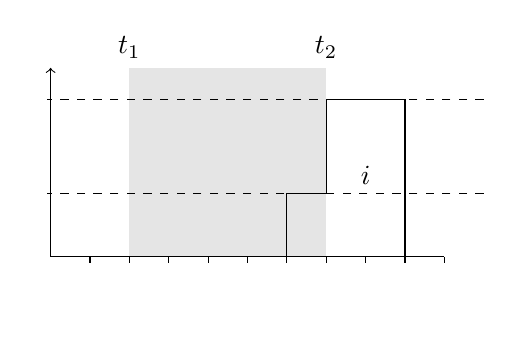
\begin{tikzpicture}
      [xscale=0.5, yscale= 0.4,node distance=0.5cm]
      \fill[gray!20] (1,6) node[above,black] {$t_1$} +(0,-6)  rectangle (6,6) node[above,black] {$t_2$};
      \node (sil) at (1,0) {} ;
      \node (eil) at (8,0) {} ;
      \node [below of=eil,node distance=0.63cm]  {$\LE$};
      \draw (sil.center) node[below=0.2cm] {$\ES$};
      
      \draw (-1,0) -- (9,0);
      
      \draw[->] (-1,0) -- (-1,6);
      \draw[dashed] (10, 2) -- (1,2) -- (-1.1,2) node[left] {$\bmin$};
      \draw[dashed] (10, 5) -- (1,5) -- (-1.1,5) node[left] {$\bmax$};
      \path[draw] (8,0) -- (8,5) -- (6,5) -- (6,2) node[right=0.5cm, above]{$i$} -- (5,2) -- (5,0);


      \foreach \i in {0,...,9} {
        \draw (\i,0)  -- (\i,-0.2);
      }
    \end{tikzpicture}
}
\hfill
\subcaptionbox{Activité $j$}[0.45\linewidth]{
    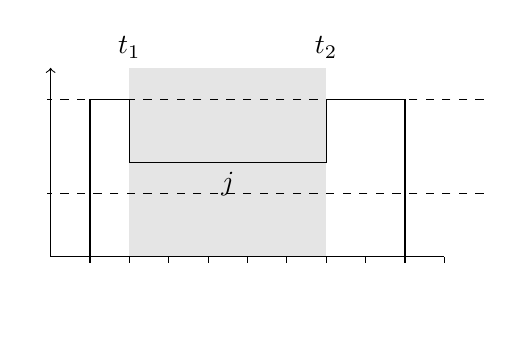
\begin{tikzpicture}
      [xscale=0.5, yscale= 0.4,node distance=0.5cm]      
      \fill[gray!20] (1,6) node[above,black] {$t_1$} +(0,-6)  rectangle (6,6) node[above,black] {$t_2$};
      \node (sil) at (0,0) {} ;
      \node (eil) at (8,0) {} ;
      \node [below of=eil,node distance=0.63cm]  {$\LE$};
      \draw (sil.center) node[below=0.2cm] {$\ES$};
      
      \draw (-1,0) -- (9,0);
      
      \draw[->] (-1,0) -- (-1,6);
      \draw[dashed] (10, 2) -- (-1,2) -- (-1.1,2) node[left] {$\bmin$};
      \draw[dashed] (10, 5) -- (-1,5) -- (-1.1,5) node[left] {$\bmax$};
      \path[draw] (8,0) -- (8,5) -- (6,5) -- (6,3)  -- (1,3) node[midway,below]
     {$j$} -- (1,5)
      -- (0,5) -- (0,0);


      \foreach \i in {0,...,9} {
        \draw (\i,0)  -- (\i,-0.2);
      }
    \end{tikzpicture}
}
  \caption{Consommation de ressource dans $[t_1,t_2[$ pour le
    \CECSP~avec fonction de rendement affine.}
\label{fig:ex_Lin}
\end{figure}
\end{ex}

Ce raisonnement peut être étendu dans le cas où $f_i$ est concave et
affine par morceaux. 

\paragraph{Fonctions concave et affine par morceaux}

Dans le cas des fonctions concaves et affines par morceaux, le
raisonnement décrit au paragraphe précédent peut être généralisé. En
effet, comme dans le cas des fonctions affines, la fonction de
rendement, $f_i(b_i(t))/b_i(t)$, est décroissante. Donc, il est
toujours préférable d'exécuter l'activité avec une consommation de
ressource aussi basse que possible. La condition selon laquelle on
peut ou non exécuter l'activité $i$ avec une consommation $b_i$ dépend
donc de la taille de l'intervalle $I$. 

Si $\bmin\neq 0$ et si l'intervalle est suffisamment grand, on va donc
exécuter l'activité à $\bmin$. Sinon, et si l'intervalle est
suffisamment grand, nous essayons d'exécuter l'activité avec une
consommation $b_i \in ]\bmin,x_2^i]$, etc. Nous rappelons que les
points $x_\ell^i$ correspondent aux points de rupture de la fonction
$f_i$. Dans le cas où $\bmin \neq 0$, l'expression de $\bb$ est
formalisée ci-dessous:
\[f_i^{-1}\left(\frac{\wb}{|I|}\right)=\left\{
    \begin{aligned}
      \bmin & \qquad & \text{si } |I| \ge \frac{\wb}{f_i(\bmin)}\\
      \frac{\wb -c_{i1}|I|}{a_{i1}|I|} & \qquad & \text{si } \frac{\wb}{f_i(\bmin)}
      > |I| > \frac{\wb}{f_i(x^i_2)} \\
      \frac{\wb -c_{i2}|I|}{a_{i2}|I|} & \qquad & \text{si }  \frac{\wb}{f_i(x^i_2)}
      \ge |I| > \frac{\wb}{f_i(x^i_3)}\\
      & \qquad \vdots& \\
      \frac{\wb -c_{iP_i}|I|}{a_{iP_i}|I|} & \qquad & \text{si }  \frac{\wb}{f_i(x^i_{P_i})}
      \ge |I| > \frac{\wb}{f_i(\bmax)}\end{aligned}
  \right.
\]
Et ceci nous donne l'expression de $\bb$ suivante:
\begin{equation}
  \bb= 
  \max \left\{b_i^{min} \frac{\wb}{f_i(b_i^{min})},
    \max_{ p \in \P_i} \left(\frac{1}{a_{ip}}(\wb-|I|c_{ip})\right)\right\}
\label{eq:conv_CECSP}
\end{equation}
Dans le cas où $\bmin=0$, nous avons: 
\[
  \bb= 
  \max_{ p \in \P_i} \left(\frac{1}{a_{ip}}(\wb-|I|c_{ip})\right)
\]
Un exemple du calcul de $\bb$ dans le cas d'une fonction $f_i$ concave
et linéaire par morceaux est décrit dans
l'exemple~\ref{ex:convPWL_CECSP}.

\begin{ex}
  \label{ex:convPWL_CECSP}
  Considérons l'activité suivante (voir figure~\ref{fig:ex_PWL}): 
  \begin{center}
  \begin{tabular}{|P{1cm}P{1cm}P{1cm}P{1cm}P{1cm}P{1cm}P{3cm}|}
    \hline
    act. & \ES & \LE & W_i & \bmin & \bmax & f_i(b)\\
    \hline
    i & 2 & 8 & 70 & 2 & 5 & 3b+1 \text{ si } b \in [2,3]\\
    &  & &  &  &  & 2b+4 \text{ si } b \in ]3,4]\\
    &  & &  &  &  & b+8 \text{ si } b \in ]4,5]\\
    \hline
  \end{tabular}
\end{center}

Si nous calculons $\wb$ et $\bb$ sur l'intervalle $[2,6[$, nous
obtenons: 
\begin{itemize}
\item $\wb[i][2][6] = \wbRS[i][2][6]  = 44$ et 
\item $\begin{aligned}[t]
        \bb[i][2][6]  &= 
  \max (\bmin \frac{ \wb[i][2][6] }{f_i(\bmin)},
  \max_{p  \in \{1,2,3\}} \frac{1}{a_{ip}} ( \wb[i][2][6] 
  - c_{ip} |I|)) \\
  &=\max  \left(2 \frac{44}{7}, \max\left\{\frac{1}{3} ( 44
  - 4) , \frac{1}{2} (44  - 4 \times 4 ), \frac{1}{1} (44  - 8 \times 4 )
\right\}\right) \\ &=  
\max ( \frac{88}{7},
\max\{\frac{40}{3}, 14, 12 \}) \\ &= 14 \end{aligned}$

~

\end{itemize}
Dans ce cas, c'est la seconde partie de la fonction $f_i$ qui est
utilisée, i.e. $f_i(b)=2b+4 \text{ si } b \in ]3,4]$.

Si maintenant nous calculons $\wb$ et $\bb$ sur l'intervalle $[4,6[$,
nous obtenons: 
\begin{itemize}
\item $\wb[i][4][6] = \wbCS[j][4][6] =18$ et 

\item $\begin{aligned}[t]
  \bb[i][4][6] &=\max (\bmin \frac{ \wb[i][4][6] }{f_i(\bmin)},
  \max_{p  \in \{1,2,3\}} \frac{1}{a_{ip}} ( \wb[i][4][6] 
  - c_{ip} |I|)) \\
  &=\max  \left(2 \frac{18}{7}, \max\left\{\frac{1}{3} ( 18
      - 2) , \frac{1}{2} (18  - 4 \times 2), \frac{1}{1} (18  - 8 \times 2 )
    \right\}\right) \\ &=  
  \max ( \frac{36}{7},
  \max\{\frac{16}{3}, 5 , 2 \}) \\ &= \frac{16}{3} 
\end{aligned}$

~

\end{itemize}
Et dans ce cas, c'est la première partie de la fonction $f_i$ qui est
utilisée, i.e. $f_i(b)=3b+1 \text{ si } b \in ]2,3]$.

\begin{figure}[!htb]
  \centering
  \subcaptionbox{Consommation minimale sur $[2,6[$}[0.45\linewidth]{
    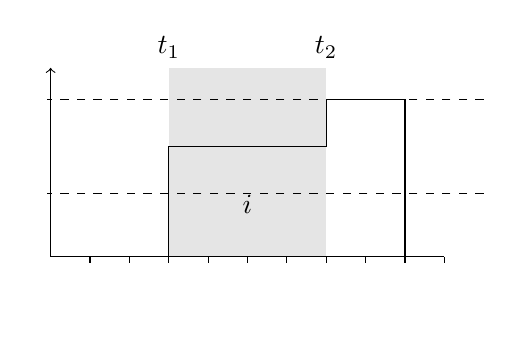
\begin{tikzpicture}
      [xscale=0.5, yscale= 0.4,node distance=0.5cm]
      \fill[gray!20] (2,6) node[above,black] {$t_1$} +(0,-6)  rectangle (6,6) node[above,black] {$t_2$};
      \node (sil) at (2,0) {} ;
      \node (eil) at (8,0) {} ;
      \node [below of=eil,node distance=0.63cm]  {$\LE$};
      \draw (sil.center) node[below=0.2cm] {$\ES$};
      
      \draw (-1,0) -- (9,0);
      
      \draw[->] (-1,0) -- (-1,6);
      \draw[dashed] (10, 2) -- (-1,2) -- (-1.1,2) node[left] {$\bmin$};
      \draw[dashed] (10, 5) -- (-1,5) -- (-1.1,5) node[left] {$\bmax$};
      \path[draw] (8,0) -- (8,5) -- (6,5) -- (6,3.5)  -- (2,3.5)
      node[midway, below=0.5cm]{$i$} -- (2,0) ;


      \foreach \i in {0,...,9} {
        \draw (\i,0)  -- (\i,-0.2);
      }
    \end{tikzpicture}
}
\hfill
\subcaptionbox{Consommation minimale sur $[4,6[$}[0.45\linewidth]{
    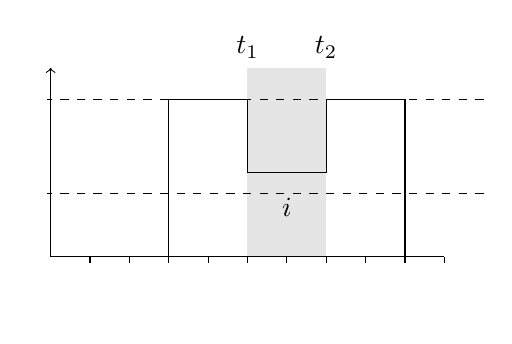
\begin{tikzpicture}
      [xscale=0.5, yscale= 0.4,node distance=0.5cm]      
      \fill[gray!20] (4,6) node[above,black] {$t_1$} +(0,-6)  rectangle (6,6) node[above,black] {$t_2$};
      \node (sil) at (2,0) {} ;
      \node (eil) at (8,0) {} ;
      \node [below of=eil,node distance=0.63cm]  {$\LE$};
      \draw (sil.center) node[below=0.2cm] {$\ES$};
      
      \draw (-1,0) -- (9,0);
      
      \draw[->] (-1,0) -- (-1,6);
      \draw[dashed] (10, 2) -- (-1,2) -- (-1.1,2) node[left] {$\bmin$};
      \draw[dashed] (10, 5) -- (-1,5) -- (-1.1,5) node[left] {$\bmax$};
      \path[draw] (8,0) -- (8,5) -- (6,5) -- (6,2.67)  -- (4,2.67) node[midway,below=0.2cm]
     {$i$} -- (4,5) -- (2,5) -- (2,0);
      -- (0,5) -- (0,0);


      \foreach \i in {0,...,9} {
        \draw (\i,0)  -- (\i,-0.2);
      }
    \end{tikzpicture}
}
  \caption{Consommation de ressource dans $[t_1,t_2[$ pour le
    \CECSP~avec fonction de rendement concave et affine par morceaux.}
\label{fig:ex_PWL}
\end{figure}
\end{ex}

\subsection{Les ajustements de bornes}
\label{sec:adjustment_tw}

Dans cette sous-section, nous décrivons les ajustements qui peuvent être
faits sur les fenêtres de temps des activités. Tout d'abord, nous
introduisons les notations suivantes: $\bbLS$ (respectivement $\bbRS$
et $\bbCS$) correspond à la quantité de ressource consommée par
l'activité $i$ dans l'intervalle $[t_1,t_2[$ quand l'activité est
calée à gauche (respectivement calée à droite et
centrée). Formellement, ces trois quantités peuvent être exprimées de
la manière suivante:
\begin{align}
  \bbLS&=   \max \left\{b_i^{min} \frac{\wbLS}{f_i(b_i^{min})},
         \max_{ p \in \P_i} \left(\frac{1}{a_{ip}}(\wbLS-|I|c_{ip})\right)\right\}\\
  \bbRS&=   \max \left\{b_i^{min} \frac{\wbRS}{f_i(b_i^{min})},
         \max_{ p \in \P_i} \left(\frac{1}{a_{ip}}(\wbRS-|I|c_{ip})\right)\right\}\\
  \bbCS&=  \max \left\{b_i^{min} \frac{\wbCS}{f_i(b_i^{min})},
         \max_{ p \in \P_i} \left(\frac{1}{a_{ip}}(\wbCS-|I|c_{ip})\right)\right\}
\end{align}

Nous allons décrire deux règles d'ajustements pour les fenêtres de
temps du \CECSP. La première permet d'ajuster $\LS$ et la seconde
$\ES$;nous avons des ajustements symétriques pour $\EE$ et $\LE$. 

Pour les premiers ajustements décrits, nous allons essayer de faire
démarrer l'activité après $t_1$ et si la quantité de ressource
disponible n’est pas suffisante pour ordonnancer les consommations
minimales de toutes les activités -– excepté celle de l’activité $i$ qui
est remplacée par $\bbRS$~–- alors, nous pouvons déduire que l’activité
doit commencer avant $t_1$.

\begin{reg}
  \label{reg:ajust_CECSP}
  S’il existe un intervalle $[t_1 , t_2 [$ avec $t_1 > \ES$ et une
  activité $i$ pour lesquels:
  \[ \sum_{\substack{j \in \A\\ j\neq i}} \bb[j] + \bbRS > R(t_2-t_1)
  \]
  alors, on a:
  \[ \LS \le t_1 - \frac{1}{\bmax}\left(\sum_{\substack{j \in \A\\ j\neq i}} \bb[j] + \bbRS - R(t_2-t_1)\right)
  \]
\end{reg}

\begin{proof}
  Soient $i$ et $[t_1,t_2[$ vérifiant la condition de la
  règle~\ref{reg:ajust_CECSP}. Supposons que l'activité $i$ démarre
  après   $t_1$. 

  La consommation minimale de $i$ dans $[t_1,t_2[$ est donc $\bbRS$. On
  a donc que $\sum_{\substack{j \in \A\\ j\neq i}} \bb[j] + \bbRS $ est
  la consommation minimale de toutes les activités dans $[t_1,t_2[$
  quand l'activité $i$ commence après $t_1$. Donc, si cette quantité est
  plus grande que la quantité de ressource disponible dans l'intervalle
  $[t_1,t_2[$, i.e. $R(t_2-t_1)$, on obtient une contradiction avec le
  fait que l'instance soit réalisable et $i$ doit commencer avant
  $t_1$. 

  Pour calculer la nouvelle date de début au plus tard de $i$,
  remarquons que la quantité de ressource devant être consommée avant
  $t_1$ est d'au moins $\sum_{\substack{j \in \A\\ j\neq i}} \bb[j] +
  \bbRS - R(t_2-t_1)$, i.e. ce qui ne ``rentrait'' pas dans
  $[t_1,t_2[$. L'objectif étant d'obtenir une borne supérieure sur la date de
  début de $i$, nous cherchons donc à exécuter cette partie de
  l'activité le plus rapidement possible. 

  Le temps minimal requis pour réaliser cette
  consommation étant obtenu en exécutant l'activité à $\bmax$, nous
  obtenons comme borne supérieure sur la date de début de $i$:
  $t_1 - 1/\bmax \times \left(\sum_{\substack{j \in \A\\ j\neq
        i}} \bb[j] + \bbRS - R(t_2-t_1)\right)$
\end{proof}

De manière similaire, nous avons les ajustements suivants sur la date
de début au plus tôt d'une activité. 
\begin{reg}
  \label{reg:ajustRi_CECSP}
  S'il existe un intervalle $[t_1,t_2[$ avec $ t_2 > \LE$ et une
  activité $i$ telle que $\bmin \neq 0$ pour lesquels:
  \[ \sum_{\substack{j \in \A \\ j \neq i}} \bb[j] +
    \min(\bbCS,\bbLS) > R (t_2-t_1)\] 
  alors
  \[ \ES \ge t_2 - \frac{1}{\bmin} \left(R (t_2-t_1) -\sum_{\substack{j
          \in \A \\ j \neq i}} \bb[j] \right) \]
\end{reg}

\begin{proof}
  Soient $i$ et $[t_1,t_2[$ vérifiant la condition de la
  règle~\ref{reg:ajust_CECSP}. Nous allons décider si $i$ peut commencer
  avant $t_1$. Les configurations où l'activité $i$ démarre avant $t_1$
  et consomme le moins de ressource possible dans $[t_1,t_2[$ sont les
  configurations où $i$ est soit calée à gauche, soit centrée.

  La consommation minimale de $i$ dans l'intervalle $[t_1,t_2[$ quand
  $i$ commence avant $t_1$ est donc $\min( \bbLS, \bbCS)$. On a donc que
  $\sum_{\substack{j \in \A\\ j\neq i}} \bb[j] + \min( \bbLS, \bbCS) $
  est la consommation minimale de toutes les activités dans $[t_1,t_2[$
  quand l'activité $i$ commence avant $t_1$. Donc, si cette quantité est
  plus grande que la quantité de ressource disponible dans l'intervalle
  $[t_1,t_2[$, i.e. $R(t_2-t_1)$, on obtient une contradiction avec le
  fait que l'instance soit réalisable et $i$ doit commencer après $t_1$.

  Pour calculer la nouvelle date de début au plus tard de $i$,
  remarquons que la quantité de ressource disponible dans $[t_1,t_2[$
  pour exécuter $i$ est de $R(t_2-t_1) -\sum_{\substack{j \in \A\\
      j\neq i}} \bb[j]$. L'objectif étant d'obtenir une borne inférieure sur la date de
  début de $i$, nous cherchons donc à ordonnancer cette partie de
  l'activité le moins rapidement possible. 

  Le temps maximal requis pour réaliser cette consommation étant
  obtenu en exécutant l'activité à $\bmin$, et, comme $\bmin \neq 0$,
  l'activité ne peut être interrompue, nous savons que l'activité doit
  être en cours à $t_2$. Nous obtenons alors comme borne inférieure sur
  la date de début de $i$:
  $t_2 - 1/\bmin \left(R (t_2-t_1) -\sum_{\substack{j
        \in \A \\ j \neq i}} \bb[j] \right) $
\end{proof}

\begin{ex}
  Considérons l'instance à $3$ activités et avec $R=5$ suivante:

  \begin{center}
    \begin{tabular}{|P{1cm}|P{1cm}P{1cm}P{1cm}P{1cm}P{1cm}P{2cm}|} 
      \hline 
      act. & \ES & \LE & W_i & \bmin& \bmax & f_i(b_i(t))\\ 
      \hline 
      1 & 0 & 6 & 28 & 1 & 5 & 2b_i(t)+1\\ 
      2 & 2 & 6 & 32 & 2 & 5 & b_i(t)+5\\ 
      3 & 2 & 5 & 6 & 2 & 2 & b_i(t)\\ 
      \hline
    \end{tabular}
  \end{center}
  Une solution réalisable est décrite par la figure~\ref{exSol}.
  \begin{figure}[!htb]
    \begin{center} 
      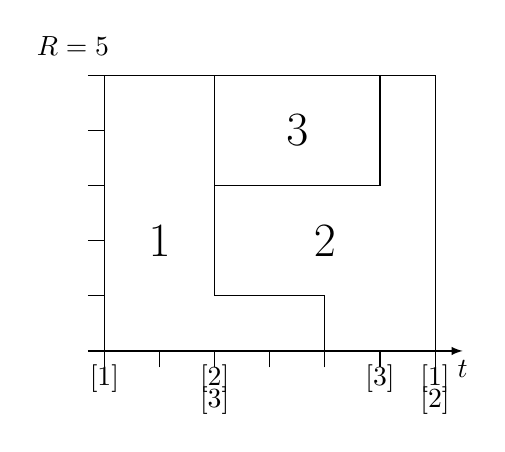
\begin{tikzpicture}
        [scale=0.7]
        \node (O) at (0,0) {};
        \node (2) at (4,2) {\LARGE $2$};
        \node (1) at (1,2) {\LARGE $1$};
        \node (3) at (3.5,4) {\LARGE $3$};
        \node[label={[shift={(-0.4,0)}]$R=5$}] (B) at (0,5) {};


        \node (r1) at (0,-0.5) {$\ES[1]$}; 
        \node (r2) at (2,-0.5) {$\ES[2]$};
        \node (r3) at (2,-0.9) {$\ES[3]$};
        \node (d1) at (6,-0.5) {$\LE[1]$};
        \node (d2) at (6,-0.9) {$\LE[2]$};
        \node (d3) at (5,-0.5) {$\LE[3]$};


        \draw[->,>=latex] (6,0) -- (6.5,0) node[below] {$t$};

        % \draw (0,0) rectangle (6,5);
        \draw (4,0) -- (6,0) -- (6,5) -- (5,5);

        \draw (2,5) -- (2,1) -- (4,1) -- (4,0) -- (0,0) -- (0,5) -- cycle;

        \draw (2,3) -- (5,3) -- (5,5) -- (2,5) ;


        \foreach \i in {0,...,5}
        {
          \draw (\i,-0.3) -- (\i,0);
          \draw (-0.3,\i) -- (0,\i);
        }

        \draw (6,-0.3) -- (6,0);

      \end{tikzpicture}
      \caption{Une solution réalisable du \CECSP.}
      \label{exSol}
    \end{center}
  \end{figure}

  Nous allons ajuster la fenêtre de temps de l'activité $1$. Pour cela,
  considérons l'intervalle $[t_1,t_2[=[2,5[$. On a:
  \begin{itemize}
  \item $\bb[2][2][5]=7$
  \item $\bb[3][2][5]=6$
  \item $\bbRS[1][2][5]=7$ et $\bbCS[1][2][5]=3$
  \end{itemize}
  Nous avons donc: $\sum_{j\in A;\ j\neq i} \bb[j][2][5] +
  \bbRS[1][2][5]= 7+7+6 =20 > 5 (5-2) =15$. Donc $\LS[1]$ peut être
  ajustée 
  à $ 2 -\frac{1}{5} (20-15) = 1$ .
  En effet, la quantité de ressource disponible dans l'intervalle
  $[2,5[$ pour ordonnancer l'activité $1$ est de $15-7-6=2$. Donc, si
  l'activité $1$ commence après $t_1$, elle ne peut consommer que $2$
  unités de ressource dans $[2,5[$.  Or, il faudrait $\bbRS[1][2][5]= 7$
  unités de ressource disponibles dans $[2,5[$ pour que $1$ puisse
  démarrer avant $t_1$. Donc l'activité $1$ ne peut commencer après $t_1$
  et, au moins $5= 7-2$ unités de ressource doivent être exécutées avant
  $t_1$. Donc $\LS[1]$ peut être ajustée à $2 - \frac{1}{5}(20-15) =1 $.

  De plus, $\LE[1]$ peut être ajusté à $t_1 + 1/ \bmin \times (R(t_2-t_1) -
  \sum_{j\in A;\ j\neq i} \bb[j] )= 2+(15-13)=4$. En effet, si l'activité
  $1$ finit après $t_2$, alors elle doit consommer au moins
  $\min(\bbRS[1][2][5],\bbCS[1][2][5])=\min(11,6)=6$ unités de ressource
  dans l'intervalle $[2,5[$. Or, seulement $2$ unités sont
  disponibles. L'activité $1$ ne peut donc pas finir après $t_2$ et nous
  pouvons ajuster $\LE[1]$ à $4$.
\end{ex}

L'algorithme~\ref{algo:ajust_CECSP} présente les ajustements pour le
\CECSP. 
\begin{algorithm}[!htb]
  \caption{Ajustement des fenêtres de temps pour le \CECSP.}
  \label{algo:ajust_CECSP}
    \PourTous {intervalles d'intérêt $[t_1,t_2[$}
    { $W\gets 0$
    
      $B\gets 0$
      \PourTous {$i \in \A$}{
        $W \gets W+\min(\wbLS,\wbCS,\wbRS)$
    
        $B \gets B+\max(\bmin\frac{W}{f_i(\bmin)},\frac{1}{a_i}(W-c_i|I|))$
      }
      \Si {$B>R(t_2-t_1)$}{
        L'instance est infaisable.}
      \Sinon{
        \PourTous {$i \in A$}{
          $W \gets \min(\wbLS,\wbCS,\wbRS)$
          
          $slack \gets R(t_2-t_1)-B+\max(\bmin\frac{W}{f_i(\bmin)},\frac{1}{a_i}(W-c_i|I|))$
    \Si {$ slack < \bbLS$}{
      $\emin \gets \max(\emin,t_2+\frac{1}{\bmax}(\bbLS-slack))$
    }
    \Si {$ slack < \min(\bbLS,\bbCS)$}{
      $\ES \gets \max(\ES,t_2-\frac{slack}{\bmin})$
    }
    \Si {$slack < \bbRS$}{
      $\smax \gets \min(\smax,t_1-\frac{1}{\bmax}(\bbRS-slack))$
    }
    \Si {$slack < \min(\bbRS,\bbCS)$}{
      $\LE \gets \min(\LE,t_1+\frac{slack}{\bmin})$
    }
  }
}
}    
\end{algorithm}


Nous avons montré qu'il était possible de calculer, étant donné un
intervalle et une activité, sa consommation minimale et les
ajustements pouvant être faits sur ses fenêtres de temps en
$O(1)$. {\'E}tant donné un intervalle, la fonction de marge ainsi que
tous les ajustements peuvent donc être calculés en $O(n)$. Dans la
sous-section suivante, nous montrons qu'il suffit d'exécuter l'algorithme
de vérification, ainsi que les ajustements sur un nombre polynomial
d'intervalles $[t_1,t_2[$.

\subsection{Caractérisation des intervalles d'intérêt}
\label{sec:intervalle_CECSP}
Dans un premier temps, nous prouvons que nous pouvons seulement
considérer un nombre polynomial d'intervalles pour détecter une
incohérence. En effet, à cause de la nature continue du problème, on
aurait pu être amené à considérer un nombre potentiellement infini
d'intervalles. 

\begin{theo}
  L'algorithme de vérification du raisonnement énergétique a seulement
  besoin d'être appliqué sur un nombre polynomial d'intervalles $[t_1,t_2[$.
\end{theo}

\begin{proof}
  La fonction de marge étant la différence entre une fonction affine,
  $R(t_2-t_1)$, et la somme de fonction affine par morceaux,
  $\bb$, c'est aussi une fonction affine par morceaux à deux
  dimensions. Le minimum de cette fonction est donc atteint en un point
  extrême d'un des polygones convexes dans lequel elle est
  affine. 

  Les segments de définitions, i.e. les segments où l'expression de la
  fonction est la même, de la fonction de marge sont les mêmes que ceux
  de la somme des consommations individuelles de chaque activité. Donc,
  d'un point de vue géométrique, un point extrême de la fonction de marge
  est l'intersection de deux segments chacun correspondant à un segment
  de définition de la fonction de consommation d'une activité. 

  Pour calculer la fonction de marge, il suffit donc d'énumérer tous
  ces points d'intersections et, pour chacun d'entre eux, d'appliquer le
  test de satisfiabilité décrit par le
  théorème~\ref{th:ER_CECSP}. Comme, pour chaque activité, il existe un
  nombre constant de segments de définition, le nombre de points
  d'intersection est de l'ordre de $O(n^2)$.
\end{proof}

De la même manière, nous pouvons prouver que les ajustements
peuvent être appliqués sur un nombre polynomial d'intervalles. Pour
cela, il suffit de considérer, à la place de la fonction de marge, la
fonction $ R(t_2-t_1) - \sum_{\substack{j \in \A\\ j \neq i}} \bb[j] -
\bbRS$ pour la règle~\ref{reg:ajust_CECSP} et $ R(t_2-t_1) - \sum_{\substack{j \in
    \A\\ j \neq i}} \bb[j] - \min(\bbCS,\bbLS)$ pour la
règle~\ref{reg:ajustRi_CECSP}. Dans la suite, nous appellerons ces
fonctions {\it fonction d'ajustement de $\LS$ et $\ES$} respectivement. 

\begin{theo}
  L'algorithme de filtrage du raisonnement énergétique a seulement
  besoin d'être appliqué sur un nombre polynomial d'intervalles $[t_1,t_2[$.
\end{theo}

Dans les paragraphes suivants, nous allons présenter trois méthodes
permettant de calculer les intervalles d'intérêt du raisonnement
énergétique. Les deux premières méthodes s'appuient sur une analyse
des segments de définition des fonctions de consommation individuelle
des activités tandis que la seconde est une adaptation du travail
de~\cite{DP} pour la contrainte cumulative et se base sur une analyse
des variations des fonctions de marge et d'ajustements.

\subsubsection{Analyse des segments de définition des fonctions de 
  consommation individuelle}

Dans ce paragraphe, nous allons donc étudier les segments de
définitions des fonctions de consommation individuelle en fonctions
des caractéristiques des activités. Plus précisément, nous devons
considérer trois cas:
\begin{itemize}
\item $\bmin=0$
\item $W_i \le f_i(\bmin)(\LE-\ES)$
\item $W_i \ge f_i(\bmin)(\LE-\ES)$
\end{itemize}
Ces trois cas devront être considérés séparément dans chacune des
méthodes proposées pour calculer les intervalles d'intérêt du
raisonnement énergétique (pour l'algorithme de vérification et les
ajustements). Cependant, seul le troisième cas sera détaillé dans
le manuscrit, les deux autres cas étant traités de manière similaire. 
% Les deux autres cas seront quant à eux détaillés dans
% l'annexe~\ref{annexe:breakline}. 

Ce raisonnement peut aussi s'appliquer pour calculer les intervalles
d'intérêt pour les ajustements mais ceci ne sera pas détaillé dans ce
manuscrit, cette méthode n'étant pas la plus efficace. De même, nous
allons seulement présenter cette technique dans le cas des fonctions
affines mais elle peut être étendues facilement au cas des fonctions
concaves et affines par morceaux. La caractérisation des intervalles
d'intérêt dans ces deux cas sera présentée dans le paragraphe suivant
et calculée à l'aide de l'analyse de la fonction de marge et des
fonctions d'ajustements. 

Pour analyser les segments de définition des fonctions de consommation
individuelle, nous allons, dans un premier temps, montrer que si nous
analysons seulement les segments de définition de $\bb$ pour $t_1 \ge
\ES$, $t_2 \le \LE$ et $t_1+t_2 \le \ES + \LE$, alors le reste des
segments peut être déduit par symétrie.

\begin{lemma}
  \label{lem:sym1}
  \[\bb=\bb[i][\ES][t_2], \ \forall t_1,t_2 \in \mathbb{R},\ t_1 \le \ES\]
  \[\bb=\bb[i][t_1][\LE], \ \forall t_1,t_2 \in \mathbb{R},\ t_2 \ge
    \LE\]
\end{lemma}

\begin{proof}
  Pour tout intervalle $[t_1,t_2[$ tel que $t_1 \le \ES$, nous avons:
  \[ \int_{t_1}^{t_2} b_i(t)dt = \int_{t_1}^{\ES} b_i(t)dt+\int_{\ES}^{t_2} b_i(t)dt\]
  Or, $b_i(t)=0, \forall t \le \ES$. Nous avons donc que:
  \[\int_{t_1}^{\ES} b_i(t)dt+\int_{\ES}^{t_2} b_i(t)dt=
    \int_{\ES}^{t_2} b_i(t)dt\]
  De plus, d'après l'expression de la consommation
  minimale~\eqref{eq:minConso}, nous avons aussi que:
  \begin{align*}
    \bb &= \min \int_{t_1}^{t_2} b_i(t)dt \\
        &=\min \int_{t_1}^{\ES} b_i(t)dt+ \min \int_{\ES}^{t_2} b_i(t)dt\\
        &= \min \int_{\ES}^{t_2} b_i(t)dt\\
        & = \bb[i][\ES][t_2]
  \end{align*}
  Nous pouvons montrer de la même manière la seconde égalité et ceci
  achève la démonstration.
\end{proof}


\begin{lemma}
  \label{lem:sym2}
  Pour tout $t_1 \ge 0,\ t_2 \ge t_1,\ \bb= \bb[i][\LE+\ES-t_2][\LE +
  \ES -t_1]$.
\end{lemma}

\begin{proof}
  Pour montrer le lemme, on peut montrer que $ \wb=
  \wb[i][\LE+\ES-t_2][\LE +\ES -t_1]$. En effet, pour une même quantité
  d'énergie, la conversion de $\wb$ en $\bb$ ne dépend que de la
  taille de l'intervalle et $\LE +\ES -t_1 - \LE - \ES+t_2 =t_2 -
  t_1$. Nous montrons donc le lemme pour $\wb$.

  \begin{itemize}
  \item $\wbLS[i][t_1'][t_2']=\max(0,W_i-f_i(\bmax)(\max(0,\LE+\ES-t_2-\ES)))=\wbRS$
    \vspace{0.2cm}
  \item $\wbRS[i][t_1'][t_2']=\max(0,W_i-f_i(f_i(\bmax))(\max(0,\LE-\LE-\ES+t_1)))=\wbLS$
  \item$
    % \setlength{\extrarowheight}{0.5cm}
    \begin{array}{rl}
      \wbCS[i][t_1'][t_2']=&\max\left(
                             \begin{array}{l}
                               f_i(\bmin) (\LE+\ES-t_1 - \ES- \LE + t_2),\\
                               W_i - f_i(\bmax)(\max(0,\LE - \LE -\ES +t_1+\\
                               \hspace{2cm}\LE +\ES - t_2 - \ES)
                             \end{array}
      \right)\\
                           & \\
      = &\max\left(
          \begin{array}{l}
            f_i(\bmin) (t_2-t_1),\\
            W_i - f_i(\bmax)(\max(0,\LE-t_2 +t_1 - \ES))
          \end{array}
      \right)\\
      = & \wbCS
    \end{array}$
  \end{itemize}
  Et donc: 
  \begin{align*}
    \wb[i][t_1'][t_2'] &=
                         \min(\wbLS[i][t_1'][t_2'],\wbCS[i][t_1'][t_2'],\wbRS[i][t_1'][t_2'])
    \\
                       & =\min(\wbRS,\wbCS,\wbLS)\\
                       & =\wb 
  \end{align*}
  avec $t_1'=\LE+\ES-t_2$ et
  $t_2'=\LE+\ES-t_1,\ \forall t_1 \le 0$ et $\forall t_2 \ge t_1$.
\end{proof}

Donc, grâce aux lemmes~\ref{lem:sym1} et~\ref{lem:sym2}, nous avons
seulement besoin d'établir l'expression de $\bb$ à l'intérieur du
polygone (triangle) délimité par les inégalités $t_1 \ge \ES, \ t_2
\le \LE,\ t_1+t_2 \le \ES+\LE$ et $ t_2 \ge t_1$. Ce triangle est
défini par les points:

$A=(\ES,\LE)$ \hfill $\ B=(\frac{\ES+\LE}{2},\frac{\ES+\LE}{2})$
\hfill $C=( \ES,\ES)$

Les différentes expressions de $\wb$ en fonction de $t_1,t_2$ et des
paramètres de l'activité $i$ sont décrits
dans~\cite{ArtiguesLopez}. Nous commençons donc par brièvement
présenter ces résultats, puis nous expliquerons comment les étendre
pour obtenir les différentes expressions de $\bb$.

Pour ce faire et pour simplifier les calculs, nous introduisons les
deux notations suivantes: $\smax$ est la borne supérieure $ \LE -
W_i/f_i(\bmax)$ sur la date de début de $i$ et $\emin$ la borne
inférieure $\ES + W_i/f_i(\bmax)$ sur la date de fin de $i$. 

Afin de décrire les zones où l'expression de $\wb$ est identique, il
faut analyser les conditions sur $t_1$ et $t_2$ selon lesquelles une
expression est choisie plutôt qu'une autre. Pour cela, les auteurs
de~\cite{ArtiguesLopez} se proposent d'étudier les segments
correspondant au cas où deux expressions ont la même valeur,
e.g. $f_i(\bmin)(t_2-t_1) = W_i - f_i(\bmax) (t_1-\ES)$. Ces segments
permettent de délimiter des zones dans lesquelles on doit décider
l'expression de $\wb$, i.e. quelle expression est minimale à
l'intérieur de cette zone. 

Par exemple, dans le cas où $W_i \ge f_i(\bmin)(\LE -\ES)$ l'unique
point pour lequel l'énergie requise est maximale est le point
$A$. Donc, $\wb[i][\ES][\LE]= W_i$ et, dans la zone délimitée par les
lignes $t_1 \le \ES$ et $t_2 \ge \LE$ (en rouge sur la
figure~\ref{fig:breakline_nrj}), l'expression de $\wb$ est $W_i$. 

Notons aussi que le cas $W_i \ge f_i(\bmin)(\LE -\ES)$ correspond au
cas où l'activité ne peut être ordonnancée à $\bmin$ durant toute sa
durée d'exécution. C'est-à-dire que l'énergie requise par l'activité
$i$ dans l'intervalle $[t_1,t_2[$ peut dépasser $f_i(\bmin)(t_2-t_1)$
et le cas où $\wb= W_i - f_i(\bmax)(\LE-t_2+t_1-\ES)$ doit être
considéré. De plus, le cas $W_i \ge f_i(\bmin)(\LE -\ES)$ est
séparé en deux sous cas: $\emin \le \smax$ et $\emin \ge \smax$. Le
premier cas correspond au cas où le point d'intersection des lignes
$t_1\le \emin$ et $t_2 \ge \smax$ vérifie $t_2 \ge t_1$ et donc le
point est à l'intérieur du triangle $(A,B,C)$. Le second cas
correspond au cas où ce point se trouve à l'extérieur du
triangle. Dans ces deux cas, les segments de définition à considérer
ne sont pas les mêmes.

Plaçons nous dans le premier cas, i.e. le cas où $\emin \le
\smax$. Dans ce cas, le segment $\overline{DD'}$ sépare les cas où
$\wb= f_i(\bmin)(t_2-t_1)$ et $\wb= W_i -
f_i(\bmax)(\LE-t_2+t_1-\ES)$, le segment $\overline{DG}$ délimite
quant à lui les zones où $\wb=f_i(\bmin)(t_2-t_1)$ et $\wb= W_i -
f_i(\bmax)(\LE-t_2)$. Les autres zones peuvent être définies de
manière similaire. Pour une analyse complète des différents
expressions de $\wb$, nous renvoyons le lecteur
à~\cite{ArtiguesLopez}. 

La figure~\ref{fig:breakline_nrj} présente ces différentes expressions
avec les expressions de $\wb$ suivantes: 
\begin{itemize}
\item la zone rouge correspond à $\underline{w}(i,t_1,t_2)=W_i$;
\item la zone verte à $\underline{w}(i,t_1,t_2)=W_i-(\LE-t_2)f_i(\bmax)$;
\item la zone bleue à $\underline{w}(i,t_1,t_2)=W_i-(t_1-\ES)f_i(\bmax)$;
\item la zone jaune à
  $\underline{w}(i,t_1,t_2)=W_i-(\LE-t_2+t_1-\ES)f_i(\bmax))$;
\item et la blanche à $\underline{w}(i,t_1,t_2)=(t_2-t_1)f_i(\bmin)$.
\end{itemize}
Les autres zones correspondent à $\underline{w}(i,t_1,t_2)=0$.

De plus, les coordonnées de chaque point sont:
\begin{itemize}
\item $A=(\ES,\LE),\ B=(\emin,\smax),\
  C=(\smax,\smax)$ and $C'=(\emin,\emin)$
\item
  $D=(\ES,\frac{\LE f_i(\bmax)-\ES f_i(\bmin)-W_i}{f_i(\bmax)-f_i(\bmin)}),\
  D'=(\frac{\ES f_i(\bmax)-\LE f_i(\bmin)+W_i}{f_i(\bmax)-f_i(\bmin)},\LE)$
\item
  $G=(\frac{\ES(f_i(\bmax)-f_i(\bmin))-\LE f_i(\bmin)+W_i}{f_i(\bmax)-2f_i(\bmin)},
  \frac{\LE(f_i(\bmax)-f_i(\bmin))-\ES f_i(\bmin)-W_i}{f_i(\bmax)-2f_i(\bmin)})$
\end{itemize}



\begin{figure}[!htb]
  \centering
  \subcaptionbox{Cas $\bmin = 0$}[0.45\linewidth]
  {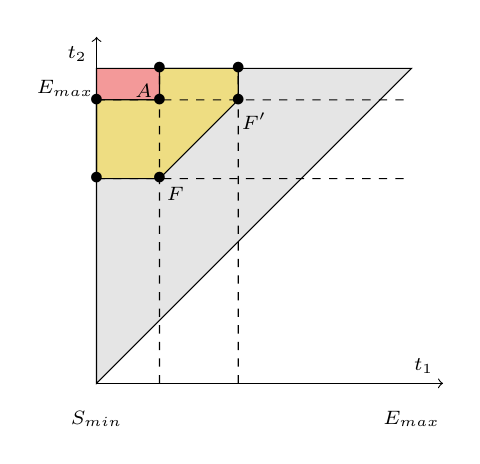
\begin{tikzpicture}
      [scale=0.4]
      \fill[gray!20] (0,0) -- (10,10) -- (0,10) -- cycle;
      \draw[fill=LightCoral!80!] (0,10) rectangle (2,9);
      \draw[fill=LightGoldenrod] (0,6.5) -- (2,6.5) -- (4.5,9) -- (4.5,10)
      -- (2,10) -- (2,9) -- (0,9) -- cycle; 
      \node (O) at (0,0) {};
      \node (T1) at (11,0) {};
      \node (T2) at (0,11) {};

      \node at (0,0) {};
      \node[label={[shift={(-0.4,-0.6)}]\scriptsize$\LE$}] (di) at (0,9) {$\bullet$};
      \node[label={[shift={(-0.4,-0.6)}]\scriptsize$E_{max}$}] at (0,10) {};

      \node[label={[shift={(0,-0.8)}]\scriptsize$S_{min}$}] at (0,0) {};
      \node[label={[shift={(0,-0.8)}]\scriptsize$\ES$}] (ri) at (2,0) {};
      \node[label={[shift={(0,-0.8)}]\scriptsize$E_{max}$}] at (10,0) {};
      \node[label={[shift={(-0.4,-0.6)}]\scriptsize$\smax$}] (smax2) at (0,6.5) {$\bullet$};

      \node[label={[shift={(0,-0.8)}]\scriptsize$\emin$}] (emin1) at (4.5,0) {};

      \node at (2,10) {$\bullet$};
      \node at (4.5,10) {$\bullet$};

      \node at (2,3) {};
      \node at (5,5) {};
      \node[label={[shift={(-0.2,-0.3)}]\scriptsize$A$}] (A) at (2,9) {$\bullet$};
      \node[label={[shift={(0.2,-0.6)}]\scriptsize$F$}] at (2,6.5) {$\bullet$};
      \node[label={[shift={(0.2,-0.7)}]\scriptsize$F'$}] at (4.5,9) {$\bullet$};
      \draw[dashed] (ri.center) -- (2,10);
      \draw[dashed] (di.center) -- (10,9);
      \path[draw] (O.center) -- (10,10) -- (0,10) -- cycle;
      \draw[dashed] (emin1.center) -- (4.5,10);
      \draw[dashed] (smax2.center) -- (10,6.5);

      \draw[->] (O.center) -- (T1.center) node[above left] {\scriptsize$t_1$};
      \draw[->] (O.center) -- (T2.center) node[below left] {\scriptsize$t_2$};
    \end{tikzpicture}}

  \vspace{0.7cm}
  Cas $ W_i \le f_i(\bmin) (\LE-\ES)$


  \subcaptionbox{$ \emin \le \smax $}[0.45\linewidth]{
    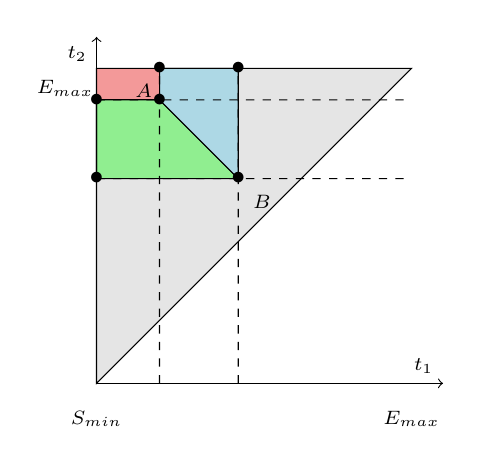
\begin{tikzpicture}
      [scale=0.4]
      % non common
      \fill[gray!20] (0,0) -- (10,10) -- (0,10) -- cycle;
      \draw[fill=LightGreen] (0,9) -- (2,9) -- (4.5,6.5) --(0,6.5) -- cycle;
      \draw[fill=LightBlue] (2,9) -- (2,10) -- (4.5,10) --(4.5,6.5) --cycle;
      \node[label={[shift={(0.3,-0.7)}]\scriptsize$B$}] (B) at (4.5,6.5) {$\bullet$};
      \node[label={[shift={(-0.4,-0.6)}]\scriptsize$\smax$}] (smax2) at (0,6.5) {$\bullet$};

      \node[label={[shift={(0,-0.8)}]\scriptsize$\emin$}] (emin1) at (4.5,0) {};
      \node at (4.5,10) {$\bullet$};
      % common

      \draw[fill=LightCoral!80!] (0,10) rectangle (2,9);
      \node (O) at (0,0) {};
      \node (T1) at (11,0) {};
      \node (T2) at (0,11) {};


      \node[label={[shift={(-0.4,-0.6)}]\scriptsize$\LE$}] (di) at (0,9) {$\bullet$};
      \node[label={[shift={(-0.4,-0.6)}]\scriptsize$E_{max}$}] at (0,10) {};

      \node[label={[shift={(0,-0.8)}]\scriptsize$S_{min}$}] at (0,0) {};
      \node[label={[shift={(0,-0.8)}]\scriptsize$\ES$}] (ri) at (2,0) {};
      \node[label={[shift={(0,-0.8)}]\scriptsize$E_{max}$}] at (10,0) {};

      \node at (2,10) {$\bullet$};

      \node[label={[shift={(-0.2,-0.3)}]\scriptsize$A$}] (A) at (2,9) {$\bullet$};

      \draw[dashed] (ri.center) -- (2,10);
      \draw[dashed] (emin1.center) -- (4.5,10);
      \draw[dashed] (di.center) -- (10,9);
      \draw[dashed] (smax2.center) -- (10,6.5);
      \path[draw] (O.center) -- (10,10) -- (0,10) -- cycle;
      \draw[->] (O.center) -- (T1.center) node[above left] {\scriptsize$t_1$};
      \draw[->] (O.center) -- (T2.center) node[below left] {\scriptsize$t_2$};
    \end{tikzpicture}}
  \hfill
  \subcaptionbox{$\emin \ge \smax$}[0.45\linewidth]{
    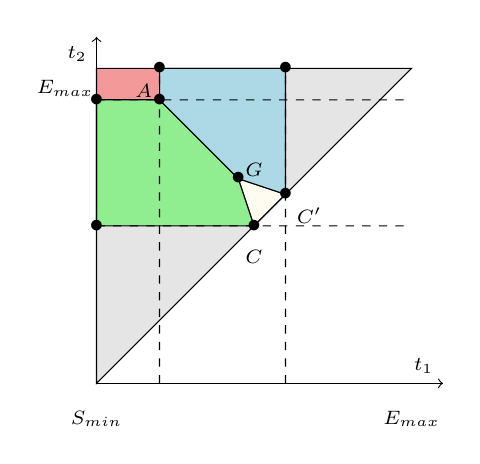
\begin{tikzpicture}
      [scale=0.4]
      \fill[gray!20] (0,0) -- (10,10) -- (0,10) -- cycle;
      \draw[fill=Cornsilk!99!black!40!] (6,6) -- (5,5) -- (4.5,6.5) -- cycle;
      \draw[fill=LightGreen] (0,9) -- (2,9)-- (4.5,6.5) -- (5,5) -- (0,5) -- cycle;
      \draw[fill=LightBlue]  (2,9) -- (2,10)-- (6,10) -- (6,6)-- (4.5,6.5) -- cycle;
      \node[label={[shift={(0,-0.8)}]\scriptsize$C$}] (C) at (5,5)  {$\bullet$};
      \node[label={[shift={(0.3,-0.7)}]\scriptsize$C'$}] (C2) at (6,6)  {$\bullet$};

      \node[label={[shift={(0.2,-0.3)}]\scriptsize$G$}] at (4.5,6.5)  {$\bullet$};
      \node[label={[shift={(-0.4,-0.6)}]\scriptsize$\smax$}] (smax2) at (0,5) {$\bullet$};

      \node[label={[shift={(0,-0.8)}]\scriptsize$\emin$}] (emin1) at (6,0) {};

      \node at (6,10) {$\bullet$};
      % common

      \draw[fill=LightCoral!80!] (0,10) rectangle (2,9);
      \node (O) at (0,0) {};
      \node (T1) at (11,0) {};
      \node (T2) at (0,11) {};

      \node[label={[shift={(-0.4,-0.6)}]\scriptsize$\LE$}] (di) at (0,9) {$\bullet$};
      \node[label={[shift={(-0.4,-0.6)}]\scriptsize$E_{max}$}] at (0,10) {};

      \node[label={[shift={(0,-0.8)}]\scriptsize$S_{min}$}] at (0,0) {};
      \node[label={[shift={(0,-0.8)}]\scriptsize$\ES$}] (ri) at (2,0) {};
      \node[label={[shift={(0,-0.8)}]\scriptsize$E_{max}$}] at (10,0) {};

      \node at (2,10) {$\bullet$};

      \node at (2,3) {};
      \node at (5,5) {};
      \node[label={[shift={(-0.2,-0.3)}]\scriptsize$A$}] (A) at (2,9) {$\bullet$};

      \draw[dashed] (ri.center) -- (2,10);
      \draw[dashed] (emin1.center) -- (6,10);
      \draw[dashed] (di.center) -- (10,9);
      \draw[dashed] (smax2.center) -- (10,5);
      \path[draw] (O.center) -- (10,10) -- (0,10) -- cycle;
      \draw[->] (O.center) -- (T1.center) node[above left] {\scriptsize$t_1$};
      \draw[->] (O.center) -- (T2.center) node[below left] {\scriptsize$t_2$};

    \end{tikzpicture}
  }

  \vspace{0.7cm}
  Cas $  W_i \ge f_i(\bmin) (\LE - \ES)$

  \subcaptionbox{$\emin \le \smax$}[0.45\linewidth]{
    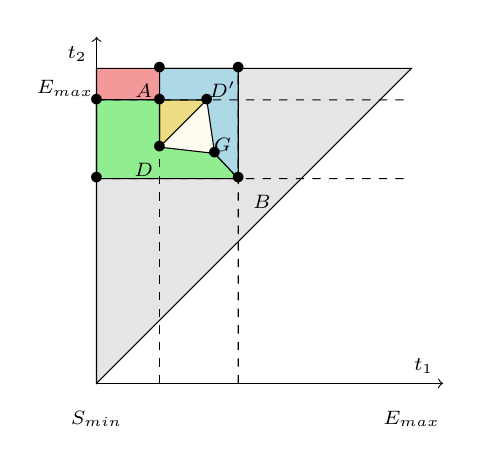
\begin{tikzpicture}
      [scale=0.4]
      % non common
      \fill[gray!20] (0,0) -- (10,10) -- (0,10) -- cycle;
      \path[fill=Cornsilk!99!black!40!] (2,7.5) -- (3.5,9)-- (3.75,7.3) -- cycle;
      \draw[fill=LightGoldenrod] (2,7.5) -- (3.5,9) -- (2,9) -- cycle;
      \draw[fill=LightGreen] (0,9) -- (2,9) -- (2,7.5)  --  (3.75,7.3) -- (4.5,6.5) -- (0,6.5)  -- (0,7.5) --cycle;
      % \draw[fill=PaleGreen!70!] (0,7.5) -- (2,7.5) -- (3.75,7.3) --
      % (4.5,6.5) -- (0,6.5) -- cycle;
      \draw[fill=LightBlue] (2,9) -- (2,10) -- (4.5,10) --  (4.5,6.5) --
      (3.75,7.3) -- (3.5,9) -- cycle;
      % \draw[fill=PowderBlue!70!] (4.5,6.5)-- (3.75,7.3) -- (3.5,9) -- (3.5,10) -- (4.5,10) --cycle;
      \node[label={[shift={(-0.2,-0.7)}]\scriptsize$D$}] (D) at (2,7.5) {$\bullet$};
      \node[label={[shift={(0.2,-0.3)}]\scriptsize$D'$}] (D2) at (3.5,9) {$\bullet$};
      \node[label={[shift={(0.1,-0.3)}]\scriptsize$G$}] (E) at (3.75,7.3)  {$\bullet$};
      \node[label={[shift={(0.3,-0.7)}]\scriptsize$B$}] (B) at (4.5,6.5) {$\bullet$};
      \node[label={[shift={(-0.4,-0.6)}]\scriptsize$\smax$}] (smax2) at (0,6.5) {$\bullet$};

      \node[label={[shift={(0,-0.8)}]\scriptsize$\emin$}] (emin1) at (4.5,0) {};
      \node at (4.5,10) {$\bullet$};
      % \node at (3.5,10) {$\bullet$};
      % \node at (0,7.5) {$\bullet$};
      % common


      \draw[fill=LightCoral!80!] (0,10) rectangle (2,9);
      \node (O) at (0,0) {};
      \node (T1) at (11,0) {};
      \node (T2) at (0,11) {};


      \node[label={[shift={(-0.4,-0.6)}]\scriptsize$\LE$}] (di) at (0,9) {$\bullet$};
      \node[label={[shift={(-0.4,-0.6)}]\scriptsize$E_{max}$}] at (0,10) {};

      \node[label={[shift={(0,-0.8)}]\scriptsize$S_{min}$}] at (0,0) {};
      \node[label={[shift={(0,-0.8)}]\scriptsize$\ES$}] (ri) at (2,0) {};
      \node[label={[shift={(0,-0.8)}]\scriptsize$E_{max}$}] at (10,0) {};

      \node at (2,10) {$\bullet$};

      \node at (2,3) {};
      \node at (5,5) {};
      \node[label={[shift={(-0.2,-0.3)}]\scriptsize$A$}] (A) at (2,9) {$\bullet$};

      \draw[dashed] (ri.center) -- (D.center);
      \draw[dashed] (emin1.center) -- (4.5,10);
      \draw[dashed] (di.center) -- (10,9);
      \draw[dashed] (smax2.center) -- (10,6.5);
      \path[draw] (O.center) -- (10,10) -- (0,10) -- cycle;
      \draw[->] (O.center) -- (T1.center) node[above left] {\scriptsize$t_1$};
      \draw[->] (O.center) -- (T2.center) node[below left] {\scriptsize$t_2$};

    \end{tikzpicture}
  }
  \hfill
  \subcaptionbox{$\emin \ge \smax$}[0.45\linewidth]{
    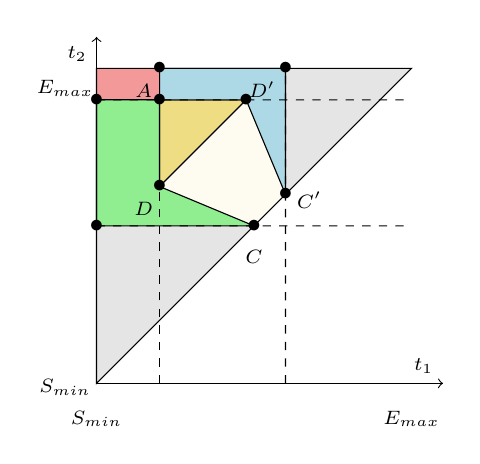
\begin{tikzpicture}
      [scale=0.4]
      % non common
      
      \fill[gray!20] (0,0) -- (10,10) -- (0,10) -- cycle;
      \path[fill=Cornsilk!99!black!40!] (2,6.25) -- (4.75,9)-- (6,6) -- (5,5) -- cycle;
      \draw[fill=LightGoldenrod] (2,6.25) -- (2,9) -- (4.75,9) -- cycle;
      \draw[fill=LightGreen] (0,9) -- (2,9) -- (2,6.25) --  (5,5)
      -- (0,5) --  cycle;
      % \draw[fill=PaleGreen!70!] (0,6.25) -- (2,6.25) -- (5,5) -- (0,5) -- cycle;
      \draw[fill=LightBlue] (2,9) -- (2,10) -- (4.75,10) -- (6,10) -- (6,6) -- (4.75,9) -- cycle;
      % \draw[fill=PowderBlue!70!] (4.75,10) -- (6,10) -- (6,6)-- (4.75,9) -- cycle;
      \node[label={[shift={(-0.2,-0.7)}]\scriptsize$D$}] (D) at (2,6.25) {$\bullet$};
      \node[label={[shift={(0.2,-0.3)}]\scriptsize$D'$}] (D2) at (4.75,9) {$\bullet$};
      \node[label={[shift={(0,-0.8)}]\scriptsize$C$}] (C) at (5,5)  {$\bullet$};
      \node[label={[shift={(0.3,-0.5)}]\scriptsize$C'$}] (C2) at (6,6)  {$\bullet$};
      \node[label={[shift={(-0.4,-0.6)}]\scriptsize$\smax$}] (smax2) at (0,5) {$\bullet$};

      \node[label={[shift={(0,-0.8)}]\scriptsize$\emin$}] (emin1) at (6,0) {};

      \node at (6,10) {$\bullet$};
      % \node at (4.75,10) {$\bullet$};
      % \node at (0,6.25) {$\bullet$};
      % common

      \draw[fill=LightCoral!80!] (0,10) rectangle (2,9);
      \node (O) at (0,0) {};
      \node (T1) at (11,0) {};
      \node (T2) at (0,11) {};

      \node[label={[shift={(-0.4,-0.4)}]\scriptsize$S_{min}$}] at (0,0) {};
      \node[label={[shift={(-0.4,-0.6)}]\scriptsize$\LE$}] (di) at (0,9) {$\bullet$};
      \node[label={[shift={(-0.4,-0.6)}]\scriptsize$E_{max}$}] at (0,10) {};

      \node[label={[shift={(0,-0.8)}]\scriptsize$S_{min}$}] at (0,0) {};
      \node[label={[shift={(0,-0.8)}]\scriptsize$\ES$}] (ri) at (2,0) {};
      \node[label={[shift={(0,-0.8)}]\scriptsize$E_{max}$}] at (10,0) {};

      \node at (2,10) {$\bullet$};

      \node at (2,3) {};
      \node at (5,5) {};
      \node[label={[shift={(-0.2,-0.3)}]\scriptsize$A$}] (A) at (2,9) {$\bullet$};

      \draw[dashed] (ri.center) -- (D.center);
      \draw[dashed] (emin1.center) -- (6,10);
      \draw[dashed] (di.center) -- (10,9);
      \draw[dashed] (smax2.center) -- (10,5);
      \path[draw] (O.center) -- (10,10) -- (0,10) -- cycle;
      \draw[->] (O.center) -- (T1.center) node[above left] {\scriptsize$t_1$};
      \draw[->] (O.center) -- (T2.center) node[below left] {\scriptsize$t_2$};

    \end{tikzpicture}

  }
  \caption{Les différentes expressions de $\wb$ en fonction des
    paramètres du problème \CECSP.}
  \label{fig:breakline_nrj}
\end{figure}

Nous avons donc défini les différentes zones correspondant chacune à
une expression de $\wb$. Dans le cas où $f_i$ est la fonction
identité, cela suffit pour définir les segments à considérer, i.e. les
segments pour lesquels on va tester l'intersection. La méthode
générale pour calculer les intervalles d'intérêt en fonction de ces
segments sera détaillée un peu plus loin dans le paragraphe. 

Les segments à considérer sont les segments délimitant deux zones avec
une expression de $\wb$ différentes, i.e. reliant deux points
représentés par une boule noire sur la
figure~\ref{fig:breakline_nrj}. Par exemple, dans le cas où $W_i \ge
f_i(\bmin)(\LE-\ES)$ les segments à considérer sont donc:
\begin{itemize}
\item dans le cas où $\emin \le \smax$: $(\ES ,E_{max})A,\ (S_{min},
  \LE)A,\ (S_{min},\smax)B,\ B(\emin,E_{max})$,  $AD,\ AD',\
  DD' ,\ DG,\ D'G$ et $GB$.
\item dans le cas où $\emin\ge \smax$: $(\ES ,E_{max})A,\ (S_{min},
  \LE)A,\ (S_{min},\smax)C,\ C'(\emin,E_{max}),\ AD$, $ AD',\
  DD' ,\ DC$ et $D'C$.
\end{itemize}
avec $D_{t_1}$ (resp. $D_{t_2}$) la projection sur l'axe $x$
(resp. sur l'axe $y$) du point $D$.


Nous allons maintenant calculer, à partir de la
figure~\ref{fig:breakline_nrj}, les zones correspondant à des
expressions différentes de $\bb$. 

Pour ce faire, nous considérons, à l'intérieur de chaque zone définie
pour $\wb$, l'inégalité suivante: 
\[ \frac{\wb}{f_i(\bmin)} \le |I|\]
avec $I=[t_1,t_2[ \cap [\ES,\LE]$. Si cette condition est vérifiée,
alors l'activité peut être ordonnancée à $\bmin$ et l'expression de
$\bb$ sera alors $\frac{\wb}{f_i(\bmin)}\times \bmin$. Dans le cas
inverse, nous avons $\bb=\frac{1}{a_i}(\wb-c_i|I|)$. 

Dans le cas où $\bmin=0$, l'inégalité n'a pas besoin d'être considérée et
nous avons directement $\bb=\frac{1}{a_i}(\wb-c_i|I|)$ dans chaque
zone. 

Dans le cas où $W_i\le f_i(\bmin)(\LE-\ES)$, $|I|$ peut valoir
$t_2-t_1$, $t_2-\ES$, $\LE-t_1$ ou $\LE-\ES$. 

Dans le premier cas,
l'inégalité donne $\wb \le f_i(\bmin)(t_2-t_1)$. Or, ce cas correspond
au cas où $[t_1,t_2[ \subset [\ES,\LE]$ et donc, $\wb=\min(W_i -
f_i(\bmax)(\LE-t_2), W_i - f_i(\bmax)(t_1-\ES),
f_i(\bmin)(t_2-t_1))$. Donc, dans ce cas, l'inégalité est toujours
vérifiée et nous avons $\bb = \bmin \times \wb/f_i(\bmin)$. 

Dans le second cas,
i.e. $|I|=t_2-\ES$, l'inégalité donne $\wb \le
f_i(\bmin)(t_2-\ES)$. Or, ce cas correspond au cas où $\wb = W_i -
f_i(\bmax)(\LE -t_2)$ , i.e. la zone verte. En remplaçant $\wb$ par
son expression, nous obtenons l'inégalité suivante: 
\[t_2 \le \frac{f_i(\bmax)\LE - f_i(\bmin)\ES - W_i }{f_i(\bmax) -
    f_i(\bmin)} \]
Or, $\LE  \le \frac{f_i(\bmax)\LE - f_i(\bmin)\ES - W_i }{f_i(\bmax) -
  f_i(\bmin)}$. Donc, l'inégalité est vérifiée si $t_2 \le d_i$
et ceci est vrai dans ce cas. 

Les cas où $|I| = \LE -\ES$ et $|I| =
\LE -t_1$ sont traités de la même façon. Donc, dans le cas où $W_i \le
f_i(\bmin) (\LE - \ES)$, $\bb=\bmin \times \wb/f_i(\bmin)$ et les
zones où $\bb$ a la même expression sont les mêmes que pour $\wb$ dans
ce cas. 

Dans le cas où $W_i \ge f_i(\bmax)(\LE - \ES)$, si $|I|$ vaut
$t_2-t_1$, l'inégalité donne $\wb \le f_i(\bmin)(t_2-t_1)$. Donc, si
$\wbCS=f_i(\bmin) (t_2-t_1)$ alors $\wb=\min(W_i -
f_i(\bmax)(\LE-t_2), W_i - f_i(\bmax)(t_1-\ES),
f_i(\bmin)(t_2-t_1))$ et l'inégalité est vérifiée. A l'inverse, si
$\wbCS=W_i - f_i(\bmax)(\LE - t_2 +t_1 - \ES)$ et comme $[t_1,t_2[
\subset [\ES,\LE]$, on a forcément $\wb=W_i - f_i(\bmax)(\LE - t_2
+t_1 - \ES)$. Donc l'inégalité n'est jamais vérifiée et
$\bb=\frac{1}{a_i}(\wb-c_i|I|)$. 

Le cas où $|I|$ vaut $t_2 - \ES$ correspond au cas où
$\wb=W_i-f_i(\bmax)(\LE-t_2)$. Dans ce cas, l'inégalité donne: 
\[ \frac{\LE f_i(\bmax) - \ES f_i(\bmin) - W_i}{f_i(\bmax)-f_i(\bmin)}
  \le t_2 \]
La partie gauche de cette inégalité correspond exactement à l'ordonnée
du point $D$ et donc la zone verte est divisée en deux parties:
\begin{itemize}
\item la partie claire où $\bb= \bmin \times \wb / f_i(\bmin)$
\item  et la partie plus foncée où $\bb=\frac{1}{a_i}(\wb - c_i|I|)$.
\end{itemize}
Les cas où $|I| = \LE -\ES$ et $|I| = \LE -t_1$ sont traités de la
même façon.

La figure~\ref{fig:breakline_res} présente ces résultats avec les
 expressions de $\bb$ suivantes:
 \begin{itemize}
 \item la zone rouge claire correspond à $\bb=\bmin \times W_i/f_i(\bmin)$;
 \item la zone rouge foncée correspond à $\bb=\frac{1}{a_i}(W_i - c_i (\LE - \ES))$;
 \item la zone verte claire à $\bb=\bmin \times
   \left\{W_i-(\LE-t_2)f_i(\bmax)\right\}/ f_i(\bmin)$;
 \item la zone verte foncée à
   $\bb=\frac{1}{a_i}(W_i-(\LE-t_2)f_i(\bmax) - c_i |I|)$ où $I$ vaut
   $[t_1,t_2[$ ou $[\ES,t_2[$;
 \item la zone bleue claire à $\bb=\bmin \times \left\{W_i-(t_1-\ES)f_i(\bmax)\right\}/f_i(\bmin)$;
 \item la zone bleue foncée à $\bb=\frac{1}{a_i}(W_i-(t_1-\ES)f_i(\bmax) - c_i
   |I|)$ où $I$ vaut  $[t_1,t_2[$ ou $[t_1,\LE{[}$;
 \item la zone jaune à
   $\bb=\frac{1}{a_i}(W_i-(\LE-t_2+t_1-\ES)f_i(\bmax) - c_i (t_2 - t_1))$;
 \item et la blanche à $\bb=(t_2-t_1) \bmin$.
 \end{itemize}
 Les autres zones correspondent à $\bb=0$.

 Les segments à considérer sont aussi décrits par la
 figure~\ref{fig:breakline_res} et sont, par exemple, dans le cas où
 $W_i \ge f_i(\bmin) (\LE-\ES)$:
 \begin{itemize}
 \item si $\emin \le \smax$: $(\ES ,E_{max})A,\ (S_{min},
   \LE)A,\ (S_{min},\smax)B, \\B(\emin,E_{max}),\ AD,\ AD',\
   D(0,D_{t_2}),\ D'(D'_{t_1},E_{max}),\ DD' ,\ DG,\ D'G$ et $GB$.
 \item si $\emin \ge \smax$: $(\ES ,E_{max})A,\ (S_{min},
   \LE)A,\ (S_{min},\smax)C,\\ C'(\emin,E_{max}),\ AD,\ AD',\
   D(0,D_{t_2}),\ D'(D'_{t_1},E_{max}),\ DD' ,\ DC$ et $D'C$.
 \end{itemize}
avec $E_{max}=\max_{i \in \A}\{\LE\}$ et $S_{min}=\min_{i \in
  \A}\{\ES\}$. 

\begin{figure}[!htb]
  \centering
  \subcaptionbox{Cas $\bmin = 0$}[0.45\linewidth]{
    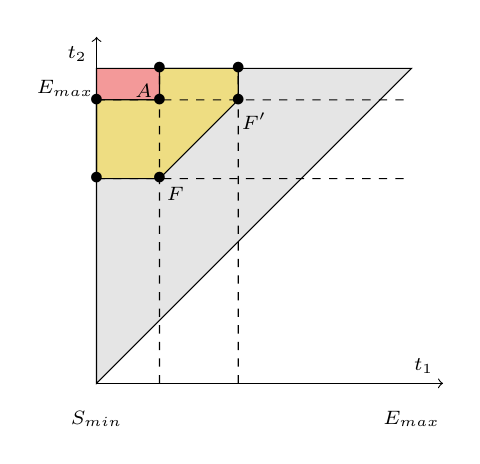
\begin{tikzpicture}
      [scale=0.4]
      \fill[gray!20] (0,0) -- (10,10) -- (0,10) -- cycle;
      \draw[fill=LightCoral!80!] (0,10) rectangle (2,9);
      \draw[fill=LightGoldenrod] (0,6.5) -- (2,6.5) -- (4.5,9) -- (4.5,10) -- (2,10) -- (2,9) -- (0,9) -- cycle;
      \node (O) at (0,0) {};
      \node (T1) at (11,0) {};
      \node (T2) at (0,11) {};
      
      \node at (0,0) {};
      \node[label={[shift={(-0.4,-0.6)}]\scriptsize$\LE$}] (di) at (0,9) {$\bullet$};
      \node[label={[shift={(-0.4,-0.6)}]\scriptsize$E_{max}$}] at (0,10) {};

      \node[label={[shift={(0,-0.8)}]\scriptsize$S_{min}$}] at (0,0) {};
      \node[label={[shift={(0,-0.8)}]\scriptsize$\ES$}] (ri) at (2,0) {};
      \node[label={[shift={(0,-0.8)}]\scriptsize$E_{max}$}] at (10,0) {};
      \node[label={[shift={(-0.4,-0.6)}]\scriptsize$\smax$}] (smax2) at (0,6.5) {$\bullet$};
      
      \node[label={[shift={(0,-0.8)}]\scriptsize$\emin$}] (emin1) at (4.5,0) {};

      \node at (2,10) {$\bullet$};
      \node at (4.5,10) {$\bullet$};

      \node at (2,3) {};
      \node at (5,5) {};
      \node[label={[shift={(-0.2,-0.3)}]\scriptsize$A$}] (A) at (2,9) {$\bullet$};
      \node[label={[shift={(0.2,-0.6)}]\scriptsize$F$}] at (2,6.5) {$\bullet$};
      \node[label={[shift={(0.2,-0.7)}]\scriptsize$F'$}] at (4.5,9) {$\bullet$};
      \draw[dashed] (ri.center) -- (2,10);
      \draw[dashed] (di.center) -- (10,9);
      \path[draw] (O.center) -- (10,10) -- (0,10) -- cycle;
      \draw[dashed] (emin1.center) -- (4.5,10);
      \draw[dashed] (smax2.center) -- (10,6.5);

      \draw[->] (O.center) -- (T1.center) node[above left] {\scriptsize$t_1$};
      \draw[->] (O.center) -- (T2.center) node[below left] {\scriptsize$t_2$};
    \end{tikzpicture}}

  \vspace{0.7cm}
  Cas $ W_i \le f_i(\bmin) (\LE-\ES)$


  \subcaptionbox{$ \emin \le \smax $}[0.45\linewidth]{
    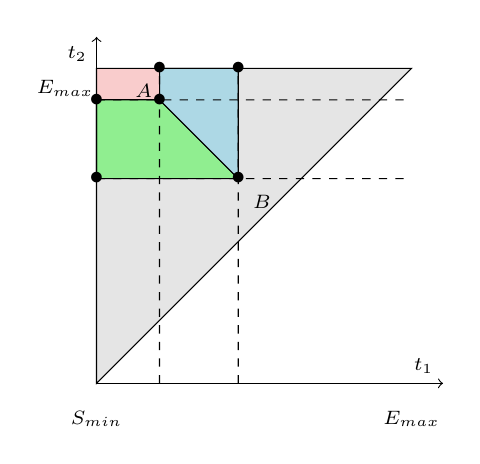
\begin{tikzpicture}
      [scale=0.4]
      \fill[gray!20] (0,0) -- (10,10) -- (0,10) -- cycle;
      % non common
      \draw[fill=LightGreen] (0,9) -- (2,9) -- (4.5,6.5) --(0,6.5) -- cycle;
      \draw[fill=LightBlue] (2,9) -- (2,10) -- (4.5,10) --(4.5,6.5) --cycle;
      \node[label={[shift={(0.3,-0.7)}]\scriptsize$B$}] (B) at (4.5,6.5) {$\bullet$};
      \node[label={[shift={(-0.4,-0.6)}]\scriptsize$\smax$}] (smax2) at (0,6.5) {$\bullet$};

      \node[label={[shift={(0,-0.8)}]\scriptsize$\emin$}] (emin1) at (4.5,0) {};
      \node at (4.5,10) {$\bullet$};
      % common

      \draw[fill=LightCoral!40!] (0,10) rectangle (2,9);
      \node (O) at (0,0) {};
      \node (T1) at (11,0) {};
      \node (T2) at (0,11) {};


      \node[label={[shift={(-0.4,-0.6)}]\scriptsize$\LE$}] (di) at (0,9) {$\bullet$};
      \node[label={[shift={(-0.4,-0.6)}]\scriptsize$E_{max}$}] at (0,10) {};

      \node[label={[shift={(0,-0.8)}]\scriptsize$S_{min}$}] at (0,0) {};
      \node[label={[shift={(0,-0.8)}]\scriptsize$\ES$}] (ri) at (2,0) {};
      \node[label={[shift={(0,-0.8)}]\scriptsize$E_{max}$}] at (10,0) {};

      \node at (2,10) {$\bullet$};

      \node[label={[shift={(-0.2,-0.3)}]\scriptsize$A$}] (A) at (2,9) {$\bullet$};

      \draw[dashed] (ri.center) -- (2,10);
      \draw[dashed] (emin1.center) -- (4.5,10);
      \draw[dashed] (di.center) -- (10,9);
      \draw[dashed] (smax2.center) -- (10,6.5);
      \path[draw] (O.center) -- (10,10) -- (0,10) -- cycle;
      \draw[->] (O.center) -- (T1.center) node[above left] {\scriptsize$t_1$};
      \draw[->] (O.center) -- (T2.center) node[below left] {\scriptsize$t_2$};
    \end{tikzpicture}}
  \hfill
  \subcaptionbox{$\emin \ge \smax$}[0.45\linewidth]{
    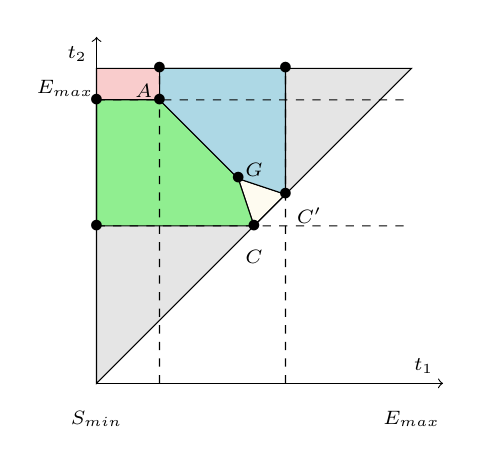
\begin{tikzpicture}
      [scale=0.4]
      \fill[gray!20] (0,0) -- (10,10) -- (0,10) -- cycle;
      \draw[fill=Cornsilk!99!black!40!] (6,6) -- (5,5) -- (4.5,6.5) -- cycle;
      \draw[fill=LightGreen] (0,9) -- (2,9)-- (4.5,6.5) -- (5,5) -- (0,5) -- cycle;
      \draw[fill=LightBlue]  (2,9) -- (2,10)-- (6,10) -- (6,6)-- (4.5,6.5) -- cycle;
      \node[label={[shift={(0,-0.8)}]\scriptsize$C$}] (C) at (5,5)  {$\bullet$};
      \node[label={[shift={(0.3,-0.7)}]\scriptsize$C'$}] (C2) at (6,6)  {$\bullet$};

      \node[label={[shift={(0.2,-0.3)}]\scriptsize$G$}] at (4.5,6.5)  {$\bullet$};
      \node[label={[shift={(-0.4,-0.6)}]\scriptsize$\smax$}] (smax2) at (0,5) {$\bullet$};

      \node[label={[shift={(0,-0.8)}]\scriptsize$\emin$}] (emin1) at (6,0) {};

      \node at (6,10) {$\bullet$};
      % common

      \draw[fill=LightCoral!40!] (0,10) rectangle (2,9);
      \node (O) at (0,0) {};
      \node (T1) at (11,0) {};
      \node (T2) at (0,11) {};

      \node[label={[shift={(-0.4,-0.6)}]\scriptsize$\LE$}] (di) at (0,9) {$\bullet$};
      \node[label={[shift={(-0.4,-0.6)}]\scriptsize$E_{max}$}] at (0,10) {};

      \node[label={[shift={(0,-0.8)}]\scriptsize$S_{min}$}] at (0,0) {};
      \node[label={[shift={(0,-0.8)}]\scriptsize$\ES$}] (ri) at (2,0) {};
      \node[label={[shift={(0,-0.8)}]\scriptsize$E_{max}$}] at (10,0) {};

      \node at (2,10) {$\bullet$};

      \node at (2,3) {};
      \node at (5,5) {};
      \node[label={[shift={(-0.2,-0.3)}]\scriptsize$A$}] (A) at (2,9) {$\bullet$};

      \draw[dashed] (ri.center) -- (2,10);
      \draw[dashed] (emin1.center) -- (6,10);
      \draw[dashed] (di.center) -- (10,9);
      \draw[dashed] (smax2.center) -- (10,5);
      \path[draw] (O.center) -- (10,10) -- (0,10) -- cycle;
      \draw[->] (O.center) -- (T1.center) node[above left] {\scriptsize$t_1$};
      \draw[->] (O.center) -- (T2.center) node[below left] {\scriptsize$t_2$};

    \end{tikzpicture}
  }

  \vspace{0.7cm}
  Cas $  W_i \ge f_i(\bmin) (\LE - \ES)$

  \subcaptionbox{$\emin \le \smax$}[0.45\linewidth]{
    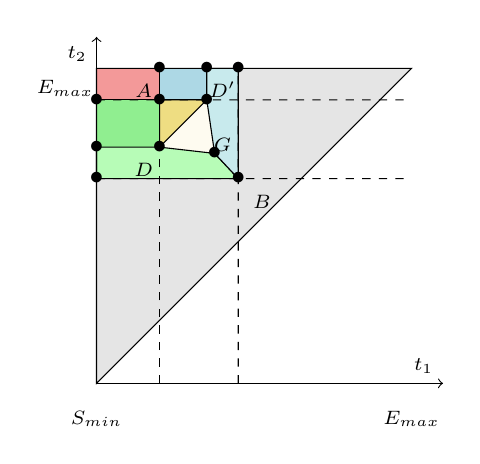
\begin{tikzpicture}
      [scale=0.4]
      % non common
      \fill[gray!20] (0,0) -- (10,10) -- (0,10) -- cycle;
      \path[fill=Cornsilk!99!black!40!] (2,7.5) -- (3.5,9)-- (3.75,7.3) -- cycle;
      \draw[fill=LightGoldenrod] (2,7.5) -- (3.5,9) -- (2,9) -- cycle;
      \draw[fill=LightGreen] (0,9) -- (2,9) -- (2,7.5) -- (0,7.5) --cycle;
      \draw[fill=PaleGreen!70!] (0,7.5) -- (2,7.5) -- (3.75,7.3) -- (4.5,6.5) -- (0,6.5) -- cycle;
      \draw[fill=LightBlue] (2,9) -- (2,10) -- (3.5,10) --(3.5,9)--cycle;
      \draw[fill=PowderBlue!70!] (4.5,6.5)-- (3.75,7.3) -- (3.5,9) -- (3.5,10) -- (4.5,10) --cycle;
      \node[label={[shift={(-0.2,-0.7)}]\scriptsize$D$}] (D) at (2,7.5) {$\bullet$};
      \node[label={[shift={(0.2,-0.3)}]\scriptsize$D'$}] (D2) at (3.5,9) {$\bullet$};
      \node[label={[shift={(0.1,-0.3)}]\scriptsize$G$}] (E) at (3.75,7.3)  {$\bullet$};
      \node[label={[shift={(0.3,-0.7)}]\scriptsize$B$}] (B) at (4.5,6.5) {$\bullet$};
      \node[label={[shift={(-0.4,-0.6)}]\scriptsize$\smax$}] (smax2) at (0,6.5) {$\bullet$};

      \node[label={[shift={(0,-0.8)}]\scriptsize$\emin$}] (emin1) at (4.5,0) {};
      \node at (4.5,10) {$\bullet$};
      \node at (3.5,10) {$\bullet$};
      \node at (0,7.5) {$\bullet$};
      % common

      \draw[fill=LightCoral!80!] (0,10) rectangle (2,9);
      \node (O) at (0,0) {};
      \node (T1) at (11,0) {};
      \node (T2) at (0,11) {};


      \node[label={[shift={(-0.4,-0.6)}]\scriptsize$\LE$}] (di) at (0,9) {$\bullet$};
      \node[label={[shift={(-0.4,-0.6)}]\scriptsize$E_{max}$}] at (0,10) {};

      \node[label={[shift={(0,-0.8)}]\scriptsize$S_{min}$}] at (0,0) {};
      \node[label={[shift={(0,-0.8)}]\scriptsize$\ES$}] (ri) at (2,0) {};
      \node[label={[shift={(0,-0.8)}]\scriptsize$E_{max}$}] at (10,0) {};

      \node at (2,10) {$\bullet$};

      \node at (2,3) {};
      \node at (5,5) {};
      \node[label={[shift={(-0.2,-0.3)}]\scriptsize$A$}] (A) at (2,9) {$\bullet$};

      \draw[dashed] (ri.center) -- (D.center);
      \draw[dashed] (emin1.center) -- (4.5,10);
      \draw[dashed] (di.center) -- (10,9);
      \draw[dashed] (smax2.center) -- (10,6.5);
      \path[draw] (O.center) -- (10,10) -- (0,10) -- cycle;
      \draw[->] (O.center) -- (T1.center) node[above left] {\scriptsize$t_1$};
      \draw[->] (O.center) -- (T2.center) node[below left] {\scriptsize$t_2$};

    \end{tikzpicture}
  }
  \hfill
  \subcaptionbox{$\emin \ge \smax$}[0.45\linewidth]{
    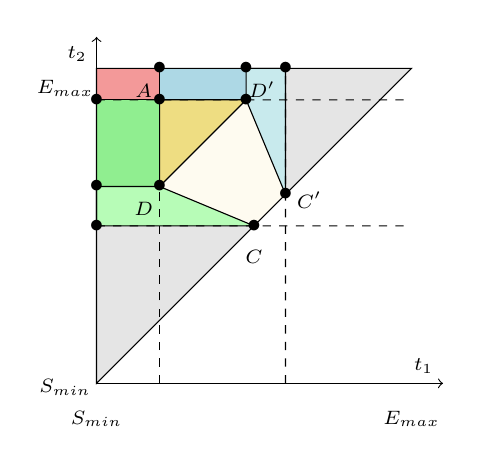
\begin{tikzpicture}
      [scale=0.4]
      % non common
      \fill[gray!20] (0,0) -- (10,10) -- (0,10) -- cycle;
      \path[fill=Cornsilk!99!black!40!] (2,6.25) -- (4.75,9)-- (6,6) -- (5,5) -- cycle;
      \draw[fill=LightGoldenrod] (2,6.25) -- (2,9) -- (4.75,9) -- cycle;
      \draw[fill=LightGreen] (0,9) -- (2,9) -- (2,6.25) -- (0,6.25) -- cycle;
      \draw[fill=PaleGreen!70!] (0,6.25) -- (2,6.25) -- (5,5) -- (0,5) -- cycle;
      \draw[fill=LightBlue] (2,9) -- (2,10) -- (4.75,10) -- (4.75,9) -- cycle;
      \draw[fill=PowderBlue!70!] (4.75,10) -- (6,10) -- (6,6)-- (4.75,9) -- cycle;
      \node[label={[shift={(-0.2,-0.7)}]\scriptsize$D$}] (D) at (2,6.25) {$\bullet$};
      \node[label={[shift={(0.2,-0.3)}]\scriptsize$D'$}] (D2) at (4.75,9) {$\bullet$};
      \node[label={[shift={(0,-0.8)}]\scriptsize$C$}] (C) at (5,5)  {$\bullet$};
      \node[label={[shift={(0.3,-0.5)}]\scriptsize$C'$}] (C2) at (6,6)  {$\bullet$};
      \node[label={[shift={(-0.4,-0.6)}]\scriptsize$\smax$}] (smax2) at (0,5) {$\bullet$};

      \node[label={[shift={(0,-0.8)}]\scriptsize$\emin$}] (emin1) at (6,0) {};

      \node at (6,10) {$\bullet$};
      \node at (4.75,10) {$\bullet$};
      \node at (0,6.25) {$\bullet$};
      % common

      \draw[fill=LightCoral!80!] (0,10) rectangle (2,9);
      \node (O) at (0,0) {};
      \node (T1) at (11,0) {};
      \node (T2) at (0,11) {};

      \node[label={[shift={(-0.4,-0.4)}]\scriptsize$S_{min}$}] at (0,0) {};
      \node[label={[shift={(-0.4,-0.6)}]\scriptsize$\LE$}] (di) at (0,9) {$\bullet$};
      \node[label={[shift={(-0.4,-0.6)}]\scriptsize$E_{max}$}] at (0,10) {};

      \node[label={[shift={(0,-0.8)}]\scriptsize$S_{min}$}] at (0,0) {};
      \node[label={[shift={(0,-0.8)}]\scriptsize$\ES$}] (ri) at (2,0) {};
      \node[label={[shift={(0,-0.8)}]\scriptsize$E_{max}$}] at (10,0) {};

      \node at (2,10) {$\bullet$};

      \node at (2,3) {};
      \node at (5,5) {};
      \node[label={[shift={(-0.2,-0.3)}]\scriptsize$A$}] (A) at (2,9) {$\bullet$};

      \draw[dashed] (ri.center) -- (D.center);
      \draw[dashed] (emin1.center) -- (6,10);
      \draw[dashed] (di.center) -- (10,9);
      \draw[dashed] (smax2.center) -- (10,5);
      \path[draw] (O.center) -- (10,10) -- (0,10) -- cycle;
      \draw[->] (O.center) -- (T1.center) node[above left] {\scriptsize$t_1$};
      \draw[->] (O.center) -- (T2.center) node[below left] {\scriptsize$t_2$};

    \end{tikzpicture}
  }
  \caption{Les différentes expressions de $\bb$ en fonction des
    paramètres du problème \CECSP.}
  \label{fig:breakline_res}
\end{figure}

Pour calculer les intervalles d'intérêt pour l'algorithme de
vérification du raisonnement énergétique, il faut, pour chaque paire
de segments de définition, calculer leur point d'intersection, s'il
existe. Les coordonnées de ce point d'intersection correspondent à un
intervalle d'intérêt. 

Pour calculer ces points d'intersection, deux méthodes existent. La
première est la plus naïve et consiste à considérer toutes les paires
de segments et calculer leur intersection. La seconde méthode utilise
l'algorithme de balayage de Bentley-Ottmann~\cite{sweep}.  L'idée
principale sur laquelle repose l'algorithme de balayage est que deux
segments ne peuvent s'intersecter si leurs projections sur l'axe
des ordonnées et sur l'axe des abscisses ne se chevauchent pas. Une
ligne horizontale fictive est utilisée pour balayer l'axe des
abscisses et à certains ``événements'', on teste l'intersection entre
deux segments s'ils intersectent tous les deux cette ligne fictive et
s'ils sont consécutifs dans l'ordre vertical. Avec cet algorithme, le
nombre de tests d'intersection peut grandement décroître par rapport à
l'algorithme naïf.

Dans le cas de l'algorithme naïf, la complexité totale de l'algorithme
de vérification est de $O(n^3)$ tandis que, pour l'algorithme de
balayage la complexité est de $O((n^2+nk) \log n)$, avec $k$ le nombre
de points d'intersection. En théorie, la complexité du second
algorithme peut être plus élevée ($k$ peut être de l'ordre de
$O(n^2)$), mais en pratique, cette complexité peut devenir très faible
si le nombre de points d'intersection est petit. Une comparaison de
ces deux algorithmes sera effectué dans le chapitre~\ref{sec:expe}.

\subsubsection{Analyses des variations de la fonction de marge et des
  fonctions d'ajustements}

Nous allons décrire ici une troisième méthode permettant le calcul des
intervalles d'intérêt du raisonnement énergétique. Cette méthode est
l'adaptation des travaux de~\cite{DP} dans le cadre du \CUSP. Dans un
premier temps, nous décrivons la méthode permettant de calculer ces
intervalles pour l'algorithme de vérification, puis nous présenterons
ce même résultat dans le cadre des ajustements de fenêtres de temps. 

 La méthode décrite dans ce paragraphe repose sur le fait que, pour
 chercher un intervalle $[t_1,t_2[$ vérifiant $SL(t_1,t_2) < 0$, il
 suffit de s'intéresser au point $(t_1,t_2)$ pour lesquels la
 fonction de marge est minimale. Comme, en pratique, il est difficile
 de trouver le minimum global d'une telle fonction, nous nous
 intéressons à ces minima locaux. Grâce au test de la dérivée
 seconde (voir sous-section~\ref{sec:nrj_CUSP}), nous pouvons dériver
 des conditions selon lesquels $SL$ est localement minimale.

\begin{lemma}[\cite{DP}]
\label{lem:min_CECSP}
La fonction de marge $SL(t_1,t_2)$ est localement minimale seulement
s'il existe deux activités $i$ et $j$ telles que les conditions
ci-dessous sont satisfaites: 
\begin{align} \frac{\delta^{-}\bb}{\delta t_1} &>
\frac{\delta^{+}\bb}{\delta t_1} \label{eq:deriv1_CECSP}\\ 
\frac{\delta^{-}\bb[j]}{\delta t_2}
& > \frac{\delta^{+}\bb[j]}{\delta t_2} \label{eq:deriv2_CECSP}
\end{align}
\end{lemma}

Le preuve est identique à celle du lemme~\ref{lem:min_CUSP}. Le
lemme~\ref{lem:min_CECSP} peut être utilisé pour déterminer les
conditions nécessaires permettant de déterminer l'ensemble des
intervalles d'intérêt. Pour cela, une étude des fonctions $t_1
\rightarrow \bb$ et $t_2 \rightarrow \bb$ est nécessaire. 

\begin{theo}
  Pour chaque activité $i$ et pour tout début d'intervalle $t_1$ il
  existe au plus deux intervalles $[t_1,t_2[$ tels que
  $\frac{\delta^{-}\bb}{\delta t_2} >
  \frac{\delta^{+}\bb}{\delta t_2} $. 
  De même,  pour chaque activité $i$ et pour toute fin d'intervalle $t_2$, il
  existe au plus deux intervalles $[t_1,t_2[$ tels que
  $\frac{\delta^{-}\bb}{\delta t_1} >
  \frac{\delta^{+}\bb}{\delta t_1} $. 
  Ces intervalles sont décrits
  par le tableau~\ref{fig:interCheck_CECSP} avec:
  \begin{center}
    \begin{tabular}{lcr}
      $\Delta'(t_2)=\frac{t_2(f_i(\bmin)-f_i(\bmax))+\LE f_i(\bmax)-W_i}{f_i(\bmin)}$
      & ;
      &$\Gamma'(t_2)=\frac{W_i-t_2f_i(\bmin)+\ES f_i(\bmax)}{f_i(\bmax)-f_i(\bmin)}$
    \end{tabular}
  \end{center}

les points de cassures de la fonction $t_1 \rightarrow \bb$ et 

\begin{center}
\begin{tabular}{lcr}
  $\Gamma(t_1)=\frac{W_i-t_1(f_i(\bmin)-f_i(\bmax))+\ES f_i(\bmax)}{f_i(\bmin)}$&
  ;
  &$\Delta(t_1)=\frac{W_i-f_i(\bmin)\LE +t_1f_i(\bmax)}{f_i(\bmax)-f_i(\bmin)}$
\end{tabular}
\end{center}

de la fonction $t_2 \rightarrow \bb$.

\begin{table} 
  \subcaptionbox{$t_2$ vérifiant~\eqref{eq:deriv2_CECSP}\label{tab:interCheck_t2}}[0.45\linewidth]{
{\rotatebox{90}{\small
    \begin{tabular}{|>{\centering\arraybackslash}m{1.7cm}|>{\centering\arraybackslash}m{1.7cm}|>{\centering\arraybackslash}m{1.5cm}|>{\centering\arraybackslash}m{1.4cm}|>{\centering\arraybackslash}m{1.4cm}|>{\centering\arraybackslash}m{1.7cm}|>{\centering\arraybackslash}m{1.4cm}|>{\centering\arraybackslash}m{1.4cm}|>{\centering\arraybackslash}m{1.4cm}|>{\centering\arraybackslash}m{1.5cm}|}
      \hline
      \rule[-0.8em]{0pt}{2em} $\bmin=0$ & 
                                          \multicolumn{4}{c|}{$W_i\le
                                          f_i(\bmin)(\LE -\ES )$} & 
                                                                    \multicolumn{5}{c|}{$W_i\ge
                                                                    f_i(\bmin)(\LE
                                                                    -\ES
                                                                    )$}\\ 
\hline 
      $t_1\le \emin$  & $t_1\le \ES $ & 
                                        \multicolumn{3}{c|}{$\ES \le
                                        t_1\le \emin$} & $t_1\le \ES
                                                         $& 
                                                                                                     \multicolumn{4}{c|}{$\ES
                                                                                                     \le
                                                                                                     t_1\le
                                                                                                     \emin$}\\ 
      \cline{3-5}
      \cline{7-10}
                                        & &{\rotatebox{-90}{$\emin \le
                                            \smax$ xor $t_1\le \htu$}}
                      & {\rotatebox{-90}{$t_1\ge \smax$}} &
                                                            {\rotatebox{-90}{$\emin>\smax$
                                                            et $\smax
                                                            > t_1
                                                            >
                                                            \htu$}} &
                                                          &
                                                            {\rotatebox{-90}{$t_1
                                                            > \itu$ et
                                                            $t_1 <
                                                            \smax$ et
                                                            $t_1 <
                                                            \htu$~}}
                                        & {\rotatebox{-90}{$t_1\le
                                          \itu$}} &
                                                    {\rotatebox{-90}{$t_1
                                                    \ge \smax$ et
                                                    $\emin \ge
                                                    \smax$}} &
                                                               {\rotatebox{-90}{$t_1
                                                               \ge
                                                               \htu$
                                                               et
                                                               $\emin
                                                               < \smax$}} \\
      \hline
      \multirow{2}{*}{$\inter[t_1][\LE ]$} &
                                             \multirow{2}{*}{$\inter[t_1][\LE
                                             ]$} & $[
                                                   t_1,\ES  $ & \multirow{2}{*}{$\inter[t_1][\bu{t_1}]$} & $\inter[t_1][\bu{t_1}]$ &\multirow{2}{*}{$\inter[t_1][\LE ]$} & $\inter[t_1][\bu{t_1}]$ & $\inter[t_1][\LE ]$ &\multirow{2}{*}{$\inter[t_1][\bu{t_1}]$}& $[
                                                   t_1,\ES  $\\
                                        & & $+\LE -t_1[$& & $\inter[t_1][\bd{t_1}]$ & & $\inter[t_1][\bd{t_1}]$ & $\inter[t_1][\bd{t_1}]$ & & $+\LE -t_1[$ \\
      \hline
    \end{tabular}
  }}
}
\hspace{0.8cm}
\subcaptionbox{$t_1$ vérifiant~\eqref{eq:deriv1_CECSP}\label{tab:interCheck_t1}}[0.45\linewidth]{
  {\rotatebox{90}{\small
      \begin{tabular}{|>{\centering\arraybackslash}m{1.7cm}|>{\centering\arraybackslash}m{1.7cm}|>{\centering\arraybackslash}m{1.5cm}|>{\centering\arraybackslash}m{1.4cm}|>{\centering\arraybackslash}m{1.4cm}|>{\centering\arraybackslash}m{1.7cm}|>{\centering\arraybackslash}m{1.4cm}|>{\centering\arraybackslash}m{1.4cm}|>{\centering\arraybackslash}m{1.4cm}|>{\centering\arraybackslash}m{1.5cm}|}
        \hline
        \rule[-0.8em]{0pt}{2em} $\bmin=0$ & \multicolumn{4}{c|}{$W_i\le f_i(\bmin)(\LE -\ES )$} & \multicolumn{5}{c|}{$W_i\ge f_i(\bmin)(\LE -\ES )$}\\
        \hline
        $t_2 \ge \smax$  & $t_2 \ge \LE $ & 
                                            \multicolumn{3}{c|}{$\LE \ge t_2\ge \smax$} & $t_2\ge \LE $&
                                                                                                         \multicolumn{4}{c|}{$\LE \ge t_2\ge \smax$}\\
        \cline{3-5}
        \cline{7-10}
                                          & &{\rotatebox{-90}{$\emin
                                              \le \smax$ xor $t_2\ge
                                              \htd$}} &
                                                        {\rotatebox{-90}{$t_2\le
                                                        \emin$}} &
                                                                   {\rotatebox{-90}{$\emin
                                                                   >
                                                                   \smax$
                                                                   et $\emin
                                                                   <
                                                                   t_2
                                                                   <
                                                                   \htd$}}
                                                                                        &
                                                                                                       &
                                                                                                         {\rotatebox{-90}{$t_2
                                                                                                         < 
                                                                                                         \itd$
                                                                                                         et
                                                                                                         $t_2
                                                                                                         >
                                                                                                         \emin$
                                                                                                         et
                                                                                                         $t_2
                                                                                                         >
                                                                                                         \htd)$~}}
                                          & {\rotatebox{-90}{$t_2\ge
                                            \itd$}} &
                                                      {\rotatebox{-90}{$\emin
                                                      < \ smax$ et $t_2 \le \emin$}} & {\rotatebox{-90}{$\emin \ge \smax $ et $t_2 \le \htd$}} \\
        \hline
        \multirow{2}{*}{$\inter[\ES ][t_2]$} & \multirow{2}{*}{$\inter[\ES ][t_2]$} & $[\ES +\LE$ & \multirow{2}{*}{$\inter[\bdp{t_2}][t_2]$} & $\inter[\bdp{t_2}][t_2]$ &\multirow{2}{*}{$\inter[\ES ][t_2]$} & $\inter[\bdp{t_2}][t_2]$ & $\inter[\ES ][t_2]$ &\multirow{2}{*}{$\inter[\bdp{t_2}][t_2]$}& $[\ES +\LE $\\
                                          & & $ -t_2,t_2[$& & $\inter[\bup{t_2}][t_2]$ & & $\inter[\bup{t_2}][t_2]$ & $\inter[\bup{t_2}][t_2]$ & &  $-t_2,t_2[$ \\
        \hline
      \end{tabular}
    }}
}






  \caption{Intervalles d'intérêt pour l'algorithme de vérification du
    raisonnement énergétique pour le \CECSP.}
  \label{fig:interCheck_CECSP}
\end{table}
\end{theo}

Notons que le cas $\bmin=\bmax$, i.e. le cas cumulatif, est inclus
dans le cas $W_i \le f_i(\bmin)(\LE - \ES )$ et que dans ce cas: 
\begin{center}
\begin{tabular}{lcr}
$\Delta'(t_2)=\smax$ & et &
$\Gamma(t_1)=\emin$
\end{tabular}
\end{center}
 \begin{proof}
Nous présentons seulement comment nous obtenons les $t_2$ pertinents
pour la huitième colonne du tableau~\ref{tab:interCheck_t2}, tous les
autres cas étant obtenus de manière similaire. La signification de
cette colonne est la suivante: si $W_i \ge f_i(\bmax)(\LE-\ES)$, $\ES
\le t_1 \le \EE$ et $t_1 \le D_{t_1}$, alors les intervalles à
considérer sont $[t_1,\LE {[}$ et $[t_1, \Gamma(t_1){[}$.

Pour prouver le lemme, nous analysons les variations de la fonction
$t_2 \rightarrow \underline{b}(i,t_1,t_2)$. Pour analyser ces
variations, nous utilisons les expressions de $\bb$ en fonction de
$t_1$ et $t_2$ décrites dans le paragraphe précédent. Pour adapter ces
zones dans le cas des fonctions concaves et affines par morceaux, il
faut déterminer, dans les zones où l'expression de $\bb$ est
$\frac{1}{a_i}(\wb - c_i|I|)$, la valeur de $\max_{p \in
\P_i}(\frac{1}{a_{ip}}(\wb - c_{ip}|I|))$. Pour ce faire, notons que
le segment $\overline{DD'}$ dans la figure~\ref{fig:breakline_res},
sépare la zone où $|I|= t_2 - t_1 \ge \wb/ f_i(\bmin)$ de la zone où
cette inégalité n'est pas vérifiée. De la même manière, nous pouvons
définir une série de segments parallèles ,
$\overline{D_{p}D_{p}^{'}}$, séparant les zones où $|I|= t_2 - t_1 \ge
\wb/f_i(x_p^i)$ et celle où cette inégalité n'est pas vérifiée,
i.e. séparant les zones où $\bb= \frac{1}{a_{ip}}(\wb -
c_{ip}(t_2-t_1))$. La figure~\ref{fig:variation} représente ces
variations.
   \begin{figure}[!htb] \begin{center}
  \begin{tikzpicture}
    [xscale=1.2,yscale=0.6]
    \node (O) at (0,0) {};
    \node (D) at (10,0) {};
    \draw[dotted] (1,0) node[below=0.15cm] {$\LS$}-- (1,8.5);
    \draw[dotted] (2,0) node[below] {$\bd{t_1}$}-- (2,8.5) ;
    \draw[dotted] (4,0) -- (4,8.5);
    \draw[dotted] (5,0) -- (5,8.5);
    \draw[dotted] (6,0) -- (6,8.5);
    \draw[dotted] (7,0) -- (7,8.5);
    \draw[dotted](8,0)node[below=0.15cm] {$\LE$} -- (8,8.5) ;
    \draw[thick] (0,1) -- (1,1);

    \draw (0.5,3.5) node[rotate=-90]  {$0$};
    \draw[draw=LightGreen!90!black!90!,ultra thick] (1,1)-- (2,3);
    \draw[ultra thick] (1.5,4.75)
    node[rotate=-90] {$\frac{\bmin}{f_i(\bmin)}(W_i-
      f_i(\bmax)(\LE-t_2))$};
    \draw[draw=Cornsilk!95!black!100!,ultra thick] (2,3) -- (4,3.5);
    \draw[ultra thick]  (3,4.25)
    node[rotate=-90]
    {$\bmin(t_2-t_1)$};
    \draw[draw=LightGoldenrod!90!black!90!,ultra thick] (4,3.5)-- (5,4);
    \draw[ultra thick] (4.5,4.25) node[rotate=-90]
    {$expr_{i1}$};
    \draw[draw=LightGoldenrod!90!black!90!,ultra thick] (6,5)-- (5,4);
    \draw[ultra thick] (5.5,4.25) node[rotate=-90]
    {$expr_{i2}$};
    \draw[draw=LightGoldenrod!90!black!90!,ultra thick] (7,6.5)-- (6,5);
    \draw[ultra thick] (6.5,4.25) node[rotate=-90]
    {$expr_{i3}$};
    \draw[draw=LightGoldenrod!90!black!90!,ultra thick] (8,8.5)-- (7,6.5);
    \draw[ultra thick] (7.5,4.25) node[rotate=-90]
    {$expr_{i4}$};
    \draw[draw=LightBlue!90!black!90!,ultra thick] (8,8.5)-- (10,8.5);
    \draw[ultra thick] (9,4.75) node[rotate=-90]
    {$\frac{1}{a_{i4}}(W_i- f_i(\bmax)(t_1-\ES) - c_{i4}(\LE-t_1))$};
    \draw[->] (O.center) -- (D.center);
  \end{tikzpicture}
\end{center}




     \caption{Intervalles d'intérêt du raisonnement énergétique du
\CECSP~dans le cas où $\ES <t_1 \le D'_{t_1}$.}
     \label{fig:variation}
   \end{figure}


Les intervalles $\inter$ pour lesquels $t_2 \rightarrow \bb$ vérifie
que sa dérivée à 
gauche est inférieure à sa dérivée à droite sont 
${[}t_1,\LE{[}$ et $[t_1,\bd{t_1}[$. En effet, comme $f_i$ est une
fonction concave et affine par morceaux, nous avons: $a_{ip} >
a_{ip+1}$ et $c_{ip} <c_{ip+1}$, et donc
$\frac{\delta^{-}expr_{ip}}{\delta t_2}<
\frac{\delta^{+}expr_{ip+1}}{\delta t_2}$.

On peut remarquer que dans la figure~\ref{fig:variation}, l'indice
de $expr_{ip}$ va seulement jusqu'à $4$. Ceci est dû à une
simplification. Dans le cas général, l'indice de $expr_{ip}$ s'arrête
au rang $\ell$ si $W_i \le f_i(x^i_{\ell +1})(\LE - \ES)$.
\end{proof}

En appliquant un raisonnement symétrique pour toute fin d'intervalle
$t_2$ fixée, nous obtenons une liste d'intervalles d'intérêt, décrite
par le lemme~\ref{listinterval}.

\begin{lemma}
  \label{listinterval} 
Soient $i$ et $j$ deux activités telles que: $W_l\ge
f_l(\bmin[l])(\LE[l]-\ES[l]),\ l=i,j$. Alors, la fonction de marge est
localement minimum seulement si $(t_1,t_2)$ correspond à l'un des
intervalles suivants:
\[ \left\{
    \begin{aligned} 
      &{[}\ES[j],\LE{]} & & \text{si } \Big(\ES[j] \le \ES \lor (\ES[j]
      \le \emin \land \ES[j] \le \itu)\Big) \land \\*
      & & &\Big(\LE \ge \LE[j] \lor (\LE \ge \smax[j] \land \LE \ge \itd)\Big)\\
      \rule[-0.8em]{0pt}{2em}      
      &{[}\Delta'(\LE),\LE{]} & & \text{si } \Big(\bdp{\LE} \le \ES \lor
      (\bdp{\LE}\le \emin \land \bdp{\LE}\le \itu)\Big) \land \\*
      & & &\LE[j] \ge \LE \ge \smax[j] \land \LE \le \itd \land \LE \ge
      \htd\\
      \rule[-0.8em]{0pt}{2em}
      &{[}\Gamma'(\LE),\LE{]} & & \text{si } \Big(\bup{\LE} \le \ES \lor
      (\bup{\LE} \le \emin \land \bup{\LE} \le \itu)\Big) \\*
      & & &\land \LE[j] \ge \LE \ge \smax[j] \land \Big(\LE \ge \emin[j]
      \lor \LE \ge E_{t_2}\Big)\\
      \rule[-0.8em]{0pt}{2em}
      &{[}\LE[j]+\ES[j]-\LE,\LE{]} & & \text{si } \Big(\LE[j]+\ES[j]-\LE \le \ES \lor
      (\LE[j]+\ES[j]-\LE \le \emin \land \\*
      & & & \LE[j]+\ES[j]-\LE \le D'_{t_1})\Big) \land \LE[j] \ge \LE
      \ge \smax[j] \land \LE\le \htd\\ 
      \rule[-0.8em]{0pt}{2em}
      &{[}\ES[j],\Gamma(\ES[j]){]} & &\text{si } \ES \le \ES[j] \le \emin \land
      \ES[j] \ge \itu \land \ES[j] \le \htu \land \\* 
      & & &\Big(\bu{\ES[j]} \ge \LE[j] \lor (\bu{\ES[j]} \ge \smax[j] \land \bu{\ES[j]} \ge
      \itd)\Big)\\
      \rule[-0.8em]{0pt}{2em}
      &{[}\ES[j],\Delta(\ES[j]){]} & &\text{si } \Big(\Delta(\ES[j]) \ge \LE[j] \lor
      (\Delta(\ES[j]) \ge \smax[j] \land \Delta(\ES[j]) \ge D_{t_2})\Big) \land
      \\* 
      & & &\ES \le \ES[j] \le \emin \land \Big(\smax \ge \ES[j] \lor \ES[j] \le
      E_{t_1}\Big)\\
      \rule[-0.8em]{0pt}{2em}
      &{[}\ES[j],\LE+\ES-\ES[j]{]} & & \text{si } \Big(\LE+\ES-\ES[j] \ge \LE[j] \lor
      (\LE+\ES-\ES[j] \ge \smax[j] \\*
& & &\land \LE+\ES-\ES[j] \ge \itd)\Big) \land 
      \ES \le \ES[j] \le \emin \land \ES[j] \ge \htu
    \end{aligned} \right.
\]
\end{lemma}

Le lemme~\ref{listinterval} présente les résultats pour le cas où $i$
et $j$ vérifient $W_l\ge f_l(\bmin[l])(\LE[l]-\ES[l]),\ l=i,j$. Les autres
cas à considérer sont:
\begin{itemize}
\item $\bmin=0$ et $\bmin[j]=0$
\item $\bmin=0$ et $W_j\le f_j(\bmin[j])(\LE[j]-\ES[j])$
\item $\bmin=0$ et $W_j\ge f_j(\bmin[j])(\LE[j]-\ES[j])$
\item $W_l\le f_l(\bmin[l])(\LE[l]-\ES[l]),\ l=i,j$
\item $W_i\ge f_i(\bmin)(\LE-\ES)$ et $W_j\ge
f_j(\bmin[j])(\LE[j]-\ES[j])$
\end{itemize} 
Ces cas peuvent être déduits de manière similaire. De plus,
l'algorithme décrit ci-dessous pour appliquer le test de
satisfiabilité du raisonnement énergétique n'utilise pas directement
cette liste.

Pour décrire cet algorithme, nous introduisons les notations
suivantes: 
\begin{itemize}
\item $O_1=\{\ES ,\ \forall i \in \A\} \cup \{\LS ,\ \forall i \in \A \, |\,
  \bmin = \bmax \} $
\item $O_2=\{\LE ,\ \forall i \in \A\} \cup \{\EE ,\ \forall i \in \A \, |\,
  \bmin = \bmax \}$
\end{itemize}

L'algorithme de détection d'incohérence est alors le suivant:
\begin{algorithm}[!htb]
\setstretch{1.35}
  \caption{Algorithme de détection d'incohérence énergétique du \CECSP.}
  \label{algo:check_CECSP}
  \PourTous {$t_1 \in O_1$}{
    \PourTous {$i \in \A$}{
      Calculer $O_{t_2}$ l'ensemble des $t_2$ vérifiant la
      condition~\eqref{eq:deriv2_CECSP} à l'aide du 
      tableau~\ref{tab:interCheck_t2}
      \PourTous {$t_2 \in O_{t_2}$}{
        \Si {$R(t_2-t_1) < \sum_{j \in \A} \bb[j]$}{
          Le problème est infaisable}
      }
    }
}  
\PourTous {$t_2 \in O_2$}{
  \PourTous {$i \in \A$}{
      Calculer $O_{t_1}$ l'ensemble des $t_1$ vérifiant la
      condition~\eqref{eq:deriv1_CECSP} à l'aide du
      tableau~\ref{tab:interCheck_t1}
      \PourTous {$t_1 \in O_{t_1}$}{
        \Si {$R(t_2-t_1) < \sum_{j \in \A} \bb[j]$}{
         Le problème est infaisable}
      }
    }
}
\end{algorithm}

L'algorithme~\ref{algo:check_CECSP} est de complexité 
$O(n^3)$. En effet, pour chaque couple d'activités $(i,j)$ au plus
deux intervalles sont considérés. La complexité est donc la même que
dans la première méthode présentée. Cependant, la constante cachée est
beaucoup plus petite dans ce cas-là. Une comparaison des performances
de chaque méthode sera présentée dans le chapitre~\ref{sec:expe}.

Nous allons maintenant montrer comment ce raisonnement peut aussi
s'appliquer dans le cas du calcul des intervalles d'intérêt pour les
ajustements. Pour ce faire, nous utilisons le
lemme~\ref{lem:min_ajust_ER_CUSP}. Comme nous avons déjà calculé les
points $t_1$ vérifiant $\frac{\delta^{-}\bb}{\delta
t_1}>\frac{\delta^{+}\bb}{\delta t_1}$ et les points $t_2$ vérifiant
$\frac{\delta^{-}\bb}{\delta t_2} >\frac{\delta^{+}\bb}{\delta
t_2}$, il suffit, pour caractériser les intervalles d'intérêt pour les
ajustements, de calculer les points $t_1$ vérifiant:
\begin{equation}
\frac{\delta^{-}\bbRS}{\delta t_1} >\frac{\delta^{+}\bbRS}{\delta
t_1}\label{eq:derivt1_CECSP} \end{equation}
et les points $t_2$ vérifiant \begin{equation}
\frac{\delta^{-}\bbRS}{\delta t_2} > \frac{\delta^{+}\bbRS}{\delta
t_2}\label{eq:derivt2_CECSP}\end{equation}
Pour cela, nous analysons les variations des fonctions $t_1
\rightarrow \bbRS$ et $t_2 \rightarrow \bbRS$. Nous allons montrer
comment cela a été fait pour $t_1 \rightarrow \bbRS$ et dans le cas où
$W_i \ge f_i(\bmin) (\LE - \ES)$, les autres cas étant déduits de
manière similaire. Le tableau~\ref{tab:interAjust_CECSP} présente 
les résultats dans ces autres cas. 


\begin{theo}
  Pour chaque activité $i$ et pour tout début d'intervalle $t_1$, il
  existe au plus deux intervalles $[t_1,t_2[$ tels que
  l'équation~\eqref{eq:derivt2_CECSP} soit vérifiée.
  De même,  pour chaque activité $i$ et pour toute fin d'intervalle $t_2$, il
  existe au plus deux intervalles $[t_1,t_2[$ tels que
  l'équation~\eqref{eq:derivt1_CECSP} soit vérifiée. 
  Ces intervalles sont décrits
  par le tableau~\ref{tab:interAjust_CECSP}.
  \begin{table}[!htb]
  \subcaptionbox{$t_2$ vérifiant~\eqref{eq:derivt2_CECSP}\label{tab:interAjust_t2}}[0.45\linewidth]{
  \small
  \begin{tabular}{|>{\centering\arraybackslash}m{1.7cm}|>{\centering\arraybackslash}m{1.7cm}|>{\centering\arraybackslash}m{1.7cm}|>{\centering\arraybackslash}m{1.7cm}|>{\centering\arraybackslash}m{1.7cm}|}
    \hline
    \rule[-0.8em]{0pt}{2em} 
    $\bmin=0$ & \multicolumn{2}{c|}{$W_i\le f_i(\bmin)(\LE -\ES )$} &
                                                                      \multicolumn{2}{c|}{$W_i\ge
                                                                      f_i(\bmin)(\LE
                                                                      -\ES
                                                                      )$}\\ 
    \hline 
    \rotatebox{-90}{$t_1 < \emin$} & \rotatebox{-90}{$ \LE > t_1 \ge \smax \lor
                                     t_1 \le \LE - W_i / f_i(\bmin)$} & \rotatebox{-90}{$t_1 < \smax
                                                                        \lor t_1 > \LE - W_i / f_i(\bmin)$} & \rotatebox{-90}{$ \LE > t_1
                                                                                                              \ge \smax \lor t_1 \le \ES $}& \rotatebox{-90}{$t_1 < \smax \lor
                                                                                                                                             t_1 > \ES $}\\
    \hline
    $\inter[t_1][\LE ]$ & $\inter[t_1][\LE ]$& $[ t_1,\bd{t_1}[ $ &
                                                                    $\inter[t_1][\LE ]$& $[ t_1,\bd{t_1}[ $ \\
    \hline
  \end{tabular}
}
\hspace{0.8cm}
\subcaptionbox{$t_1$ vérifiant~\eqref{eq:derivt1_CECSP}\label{tab:interAjust_t1}}[0.45\linewidth]{
  \small
  \begin{tabular}{|>{\centering\arraybackslash}m{1.7cm}|>{\centering\arraybackslash}m{1.7cm}|>{\centering\arraybackslash}m{1.7cm}|>{\centering\arraybackslash}m{1.7cm}|>{\centering\arraybackslash}m{1.7cm}|}
    \hline
    \rule[-0.8em]{0pt}{2em} $\bmin=0$ & 
                                        \multicolumn{2}{c|}{$W_i\le
                                        f_i(\bmin)(\LE -\ES )$} & 
                                                                  \multicolumn{2}{c|}{$W_i\ge
                                                                  f_i(\bmin)(\LE
                                                                  -\ES
                                                                  )$}\\ 
    \hline 
    \rotatebox{-90}{$t_2 > \smax$  }&\rotatebox{-90}{$ t_2 \ge \LE $}
                                                                & \rotatebox{-90}{$\LE > t_2 > \smax $} &
                                                                                                          \rotatebox{-90}{$t_2
                                                                                                          \ge \itd$}
                                                                & \rotatebox{-90}{$\itd > t_2 > \smax $}\\
    \hline
    $\inter[\ES ][t_2]$ &
                          $\inter[\ES
                          ][t_2]$& $[\bdp{t_2},t_2[  $ & $\inter[\ES
                                                         ][t_2]$& $[\bdp{t_2},t_2[  $ \\
    \hline
  \end{tabular}   
}






  \caption{Intervalles d'intérêt pour les ajustements du
    raisonnement énergétique pour le \CECSP (placement à droite).}
  \label{tab:interAjust_CECSP}
\end{table}
\end{theo}

\begin{proof}
  Nous présentons seulement comment nous obtenons les $t_2$ pertinents
dans le cas où $W_i \ge f_i(\bmax)(\LE - \ES)$, i.e. les deux dernières
colonnes du tableau~\ref{tab:interAjust_t2}. Les autres cas sont
obtenus de manière similaire. Pour prouver le lemme, nous analysons
les variations de la fonction $t_2 \rightarrow \bbRS$.


\begin{figure}[!htb]
 \subcaptionbox{Cas $t_1 \le \ES$  \label{fig:variation1}}[\linewidth] {
     \begin{tikzpicture}
    [xscale=1.2,yscale=0.6]
    \node (O) at (0,0) {};
    \node (D) at (10,0) {};
    \draw[dotted] (1,0) node[below=0.15cm] {$\LS$}-- (1,8.5);
    \draw[dotted] (7,0) node[below] {$\LE$}-- (7,8.5) ;
    \draw[dotted] (3,0) node[below] {$\itu$}-- (3,8.5);
    \draw[dotted] (4,0) -- (4,8.5);
    \draw[dotted] (5,0) -- (5,8.5);
    \draw[dotted] (6,0) -- (6,8.5);
    \draw[thick] (0,1) -- (1,1);

    \draw (0.5,3.5) node[rotate=-90]  {\scriptsize $0$};
    \draw[draw=LightGreen!90!black!90!,ultra thick] (1,1)-- (3,3.25);
    \draw[ultra thick] (2,3.5)
    node[rotate=-90,text width=4cm, align= center] {\scriptsize $\frac{\bmin}{f_i(\bmin)}(W_i-
      f_i(\bmax)(\LE-t_2))$};
    \draw[draw=PaleGreen!95!black!100!,ultra thick] (3,3.25) -- (4,3.5);
    \draw[ultra thick]  (3.5,4)
    node[rotate=-90, text width=4cm, align= center] 
    {\scriptsize $\frac{1}{a_{i1}}(W_i-
      f_i(\bmax)(\LE-t_2)- c_{i1}(t_2 - \ES))$};
    \draw[draw=PaleGreen!90!black!90!,ultra thick] (4,3.5)-- (5,4);
    \draw[ultra thick] (4.5,4) node[rotate=-90, text width=4cm, align= center]
    {\scriptsize $\frac{1}{a_{i2}}(W_i-
      f_i(\bmax)(\LE-t_2)- c_{i2}(t_2 - \ES))$};
    \draw[draw=PaleGreen!90!black!90!,ultra thick] (6,5)-- (5,4);
    \draw[ultra thick] (5.5,4) node[rotate=-90, text width=4cm, align= center]
    {\scriptsize $\frac{1}{a_{i3}}(W_i-
      f_i(\bmax)(\LE-t_2) - c_{i3}(t_2 - \ES))$};
    \draw[draw=PaleGreen!90!black!90!,ultra thick] (7,6.5)-- (6,5);
    \draw[ultra thick] (6.5,4) node[rotate=-90, text width=4cm, align= center]
    {\scriptsize $\frac{1}{a_{i4}}(W_i-
      f_i(\bmax)(\LE-t_2)- c_{i4}(t_2 - \ES))$};
    \draw[draw=Coral!90!black!90!,ultra thick] (9,6.5)-- (7,6.5);
    \draw[ultra thick] (8,4) node[rotate=-90, text width=4cm, align= center]
    {\scriptsize $\frac{1}{a_{i4}}(W_i- c_{i4}(\LE - \ES))$};
    \draw[->] (O.center) -- (D.center);
  \end{tikzpicture}



 }
 \subcaptionbox{Cas $\ES < t_1 < \smax$
   \label{fig:variation2}}[\linewidth]{
    \begin{tikzpicture}
    [xscale=1.2,yscale=0.6]
    \node (O) at (0,0) {};
    \node (D) at (10,0) {};
    \draw[dotted] (1,0) node[below=0.15cm] {$\LS$}-- (1,8.5);
    \draw[dotted] (2,0) node[below] {$\bd{t_1}$}-- (2,8.5) ;
    \draw[dotted] (4,0) -- (4,8.5);
    \draw[dotted] (5,0) -- (5,8.5);
    \draw[dotted] (6,0) -- (6,8.5);
    \draw[dotted] (7,0) -- (7,8.5);
    \draw[dotted](8,0)node[below=0.15cm] {$\LE$} -- (8,8.5) ;
    \draw[thick] (0,1) -- (1,1);

    \draw (0.5,3.5) node[rotate=-90,text width=4cm, align= center]  {\scriptsize $0$};
    \draw[draw=LightGreen!90!black!90!,ultra thick] (1,1)-- (2,3);
    \draw[ultra thick] (1.5,4.75)
    node[rotate=-90,text width=4cm, align= center] {\scriptsize $\frac{\bmin}{f_i(\bmin)}(W_i-
      f_i(\bmax)(\LE-t_2))$};
    \draw[draw=Cornsilk!95!black!100!,ultra thick] (2,3) -- (4,3.5);
    \draw[ultra thick]  (3,4.25)
    node[rotate=-90,text width=4cm, align= center]
    {\scriptsize $\bmin(t_2-t_1)$};
    \draw[draw=LightGoldenrod!90!black!90!,ultra thick] (4,3.5)-- (5,4);
    \draw[ultra thick] (4.5,4.25) node[rotate=-90,text width=4cm, align= center]
    {\scriptsize $\frac{1}{a_{i1}}(W_i- f_i(\bmax)(t_1-\ES+\LE-t_2) - c_{i1}(t_2-t_1))$};
    \draw[draw=LightGoldenrod!90!black!90!,ultra thick] (6,5)-- (5,4);
    \draw[ultra thick] (5.5,4.25) node[rotate=-90,text width=4cm, align= center]
    {\scriptsize $\frac{1}{a_{i2}}(W_i- f_i(\bmax)(t_1-\ES+\LE-t_2) - c_{i2}(t_2-t_1))$};
    \draw[draw=LightGoldenrod!90!black!90!,ultra thick] (7,6.5)-- (6,5);
    \draw[ultra thick] (6.5,4.25) node[rotate=-90,text width=4cm, align= center]
    {\scriptsize $\frac{1}{a_{i3}}(W_i- f_i(\bmax)(t_1-\ES+\LE-t_2) - c_{i3}(t_2-t_1))$};
    \draw[draw=LightGoldenrod!90!black!90!,ultra thick] (8,8.5)-- (7,6.5);
    \draw[ultra thick] (7.5,4.25) node[rotate=-90,text width=4cm, align= center]
    {\scriptsize $\frac{1}{a_{i4}}(W_i- f_i(\bmax)(t_1-\ES+\LE-t_2) - c_{i4}(t_2-t_1))$};
    \draw[draw=LightBlue!90!black!90!,ultra thick] (8,8.5)-- (10,8.5);
    \draw[ultra thick] (9,4.75) node[rotate=-90,text width=4cm, align= center]
    {\scriptsize $\frac{1}{a_{i4}}(W_i- f_i(\bmax)(t_1-\ES) - c_{i4}(\LE-t_1))$};
    \draw[->] (0,0) -- (D.center) node[below] {$t_2$};
    \draw[->] (0,0) -- (0,9) node[left] {$\bbRS$};
  \end{tikzpicture}

}
 \subcaptionbox{Cas $\smax \le  t_1 < \LE $
  \label{fig:variation3}}[\linewidth]
{  \begin{tikzpicture}
    [xscale=2.2,yscale=0.6]
    \node (O) at (0,0) {};
    \node (D) at (4.5,0) {};
    \draw[dotted] (1,0) node[below] {$\LS$}-- (1,3.5);
    \draw[dotted] (2,0) node[below] {$\LE$}-- (2,3.5) ;
    

    
    \draw[draw=LightGreen!90!black!90!,ultra thick] (1,1)-- (2,3);
    \draw[ultra thick] (1.5,2)
    node[rotate=-90] {\scriptsize $\bmin(t_2-t_1)$};
    \draw[draw=Cornsilk!95!black!100!,ultra thick] (2,3) -- (4,3);
    \draw[ultra thick]  (3,2.2)
    node[rotate=-90]
    {\scriptsize  $\bmin(\LE-t_2)$};    
    \draw[->] (0,0) -- (D.center) node[below] {$t_2$};
    \draw[->] (0,0) -- (0,4) node[left] {$\bbRS$};
  \end{tikzpicture}


}
\caption{Variation de $\bbRS$ en fonction de $t_2$.}
\end{figure}


Les intervalles $\inter$ pour lesquels $t_2 \rightarrow \bbRS$ vérifie
que sa dérivée à gauche est supérieure à sa dérivée à droite sont:
\begin{itemize}
\item $[t_1, \LE {[}$ dans le cas où $t_1 \le \ES$;
\item $[t_1, \LE {[}$ et $[t_1, \Delta(t_1) [$ dans le cas où $\ES <
  t_1 < \smax$;
\item $[t_1, \LE {[}$ dans le cas où $\smax \le t_1 < \LE$.
\end{itemize}
En simplifiant et rassemblant les cas ci-dessus, nous obtenons: \begin{itemize}
\item $[t_1, \LE {[}$ dans le cas où $t_1 < \LE$;
\item $[t_1, \Delta(t_1) [$ dans le cas où $\ES <
  t_1 < \smax$.
\end{itemize}
\end{proof}

Un raisonnement identique amène à la caractérisation des intervalles
d'intérêt pour $\bbLS$. Ces résultats sont décrits dans le
tableau~\ref{tab:interAjustLS_CECSP}.
  \begin{table}[!htb]
  \subcaptionbox{$t_2$ pour le placement à gauche}[\linewidth]{
  \small  
    \begin{tabular}{|>{\centering\arraybackslash}m{1.7cm}|>{\centering\arraybackslash}m{1.7cm}|>{\centering\arraybackslash}m{1.7cm}|>{\centering\arraybackslash}m{1.7cm}|>{\centering\arraybackslash}m{1.7cm}|}
      \hline \rule[-0.8em]{0pt}{2em} $\bmin=0$ & \multicolumn{2}{c|}{$W_i\le
                                                 f_i(\bmin)(\LE -\ES )$} & \multicolumn{2}{c|}{$W_i\ge f_i(\bmin)(\LE
                                                                           -\ES )$}\\ \hline \rotatebox{-90}{$t_1 < \emin$} & \rotatebox{-90}{$
                                                                                                                              \ES \ge t_1 $} & \rotatebox{-90}{$\emin >t_1 > \ES$} &
                                                                                                                                                                                     \rotatebox{-90}{$ \itu \ge t_1 $}& \rotatebox{-90}{$\emin >t_1 > \itu
                                                                                                                                                                                                                        $}\\ \hline $\inter[t_1][\LE ]$ & $\inter[t_1][\LE ]$& $[
                                                                                                                                                                                                                                                                               t_1,\bu{t_1}[ $ & $\inter[t_1][\LE ]$& $[ t_1,\bu{t_1}[ $ \\ \hline
    \end{tabular}
}


\subcaptionbox{$t_1$ pour le placement à gauche}[\linewidth]{  
 
    \small
    \begin{tabular}{|>{\centering\arraybackslash}m{1.7cm}|>{\centering\arraybackslash}m{1.7cm}|>{\centering\arraybackslash}m{1.7cm}|>{\centering\arraybackslash}m{1.7cm}|>{\centering\arraybackslash}m{1.7cm}|}
      \hline
      \rule[-0.8em]{0pt}{2em} $\bmin=0$ & 
                                          \multicolumn{2}{c|}{$W_i\le
                                          f_i(\bmin)(\LE -\ES )$} & 
                                                                    \multicolumn{2}{c|}{$W_i\ge
                                                                    f_i(\bmin)(\LE
                                                                    -\ES
                                                                    )$}\\ 
      \hline 
      \rotatebox{-90}{$t_2 > \smax$  }&\rotatebox{-90}{$ t_2 \ge \ES
                                        \lor t_2 \ge \ES + W_i/f_i(\bmin)$}
                                                                  & \rotatebox{-90}{$\emin < t_2 < \ES + W_i/f_i(\bmin)$} &
                                                                                                                            \rotatebox{-90}{$t_2
                                                                                                                            \ge
                                                                                                                            \LE
                                                                                                                            \lor
                                                                                                                            t_2
                                                                                                                            \le
                                                                                                                            \emin$}
                                                                  & \rotatebox{-90}{$t_2 < \LE \lor t_2 > \emin  $}\\
      \hline
      $\inter[\ES ][t_2]$ &
                            $\inter[\ES
                            ][t_2]$& $[\bup{t_2},t_2[  $ & $\inter[\ES
                                                           ][t_2]$& $[\bup{t_2},t_2[  $ \\
      \hline
    \end{tabular}  
}


  \caption{Intervalles d'intérêt pour les ajustements du
    raisonnement énergétique pour le \CECSP (placement à gauche).}
  \label{tab:interAjustLS_CECSP}
\end{table}

Comme dans le cas de l'algorithme de vérification, cette
caractérisation nous permet de définir une liste d'intervalles sur
lesquels appliquer les ajustements. Pour cela, il suffit, pour chaque
couple $(i,t_1)$ et pour chaque activité $j$, de calculer les
$t_2$ d'intérêt à l'aide du tableau~\ref{tab:interAjust_CECSP} pour
les ajustements des dates de début et à l'aide du
tableau~\ref{tab:interAjustLS_CECSP} pour 
les ajustements des dates de fin. Pour une activité $i$, le nombre
d'intervalles d'intérêt est donc au plus de $4(n-1)^2 + 2* (2n+3)$.












\section{Modèle de programmation par contraintes pour le cas discret}